\documentclass[11pt]{article}

    \usepackage[breakable]{tcolorbox}
    \usepackage{parskip} % Stop auto-indenting (to mimic markdown behaviour)
    

    % Basic figure setup, for now with no caption control since it's done
    % automatically by Pandoc (which extracts ![](path) syntax from Markdown).
    \usepackage{graphicx}
    % Keep aspect ratio if custom image width or height is specified
    \setkeys{Gin}{keepaspectratio}
    % Maintain compatibility with old templates. Remove in nbconvert 6.0
    \let\Oldincludegraphics\includegraphics
    % Ensure that by default, figures have no caption (until we provide a
    % proper Figure object with a Caption API and a way to capture that
    % in the conversion process - todo).
    \usepackage{caption}
    \DeclareCaptionFormat{nocaption}{}
    \captionsetup{format=nocaption,aboveskip=0pt,belowskip=0pt}

    \usepackage{float}
    \floatplacement{figure}{H} % forces figures to be placed at the correct location
    \usepackage{xcolor} % Allow colors to be defined
    \usepackage{enumerate} % Needed for markdown enumerations to work
    \usepackage{geometry} % Used to adjust the document margins
    \usepackage{amsmath} % Equations
    \usepackage{amssymb} % Equations
    \usepackage{textcomp} % defines textquotesingle
    % Hack from http://tex.stackexchange.com/a/47451/13684:
    \AtBeginDocument{%
        \def\PYZsq{\textquotesingle}% Upright quotes in Pygmentized code
    }
    \usepackage{upquote} % Upright quotes for verbatim code
    \usepackage{eurosym} % defines \euro

    \usepackage{iftex}
    \ifPDFTeX
        \usepackage[T1]{fontenc}
        \IfFileExists{alphabeta.sty}{
              \usepackage{alphabeta}
          }{
              \usepackage[mathletters]{ucs}
              \usepackage[utf8x]{inputenc}
          }
    \else
        \usepackage{fontspec}
        \usepackage{unicode-math}
    \fi

    \usepackage{fancyvrb} % verbatim replacement that allows latex
    \usepackage{grffile} % extends the file name processing of package graphics
                         % to support a larger range
    \makeatletter % fix for old versions of grffile with XeLaTeX
    \@ifpackagelater{grffile}{2019/11/01}
    {
      % Do nothing on new versions
    }
    {
      \def\Gread@@xetex#1{%
        \IfFileExists{"\Gin@base".bb}%
        {\Gread@eps{\Gin@base.bb}}%
        {\Gread@@xetex@aux#1}%
      }
    }
    \makeatother
    \usepackage[Export]{adjustbox} % Used to constrain images to a maximum size
    \adjustboxset{max size={0.9\linewidth}{0.9\paperheight}}

    % The hyperref package gives us a pdf with properly built
    % internal navigation ('pdf bookmarks' for the table of contents,
    % internal cross-reference links, web links for URLs, etc.)
    \usepackage{hyperref}
    % The default LaTeX title has an obnoxious amount of whitespace. By default,
    % titling removes some of it. It also provides customization options.
    \usepackage{titling}
    \usepackage{longtable} % longtable support required by pandoc >1.10
    \usepackage{booktabs}  % table support for pandoc > 1.12.2
    \usepackage{array}     % table support for pandoc >= 2.11.3
    \usepackage{calc}      % table minipage width calculation for pandoc >= 2.11.1
    \usepackage[inline]{enumitem} % IRkernel/repr support (it uses the enumerate* environment)
    \usepackage[normalem]{ulem} % ulem is needed to support strikethroughs (\sout)
                                % normalem makes italics be italics, not underlines
    \usepackage{soul}      % strikethrough (\st) support for pandoc >= 3.0.0
    \usepackage{mathrsfs}
    

    
    % Colors for the hyperref package
    \definecolor{urlcolor}{rgb}{0,.145,.698}
    \definecolor{linkcolor}{rgb}{.71,0.21,0.01}
    \definecolor{citecolor}{rgb}{.12,.54,.11}

    % ANSI colors
    \definecolor{ansi-black}{HTML}{3E424D}
    \definecolor{ansi-black-intense}{HTML}{282C36}
    \definecolor{ansi-red}{HTML}{E75C58}
    \definecolor{ansi-red-intense}{HTML}{B22B31}
    \definecolor{ansi-green}{HTML}{00A250}
    \definecolor{ansi-green-intense}{HTML}{007427}
    \definecolor{ansi-yellow}{HTML}{DDB62B}
    \definecolor{ansi-yellow-intense}{HTML}{B27D12}
    \definecolor{ansi-blue}{HTML}{208FFB}
    \definecolor{ansi-blue-intense}{HTML}{0065CA}
    \definecolor{ansi-magenta}{HTML}{D160C4}
    \definecolor{ansi-magenta-intense}{HTML}{A03196}
    \definecolor{ansi-cyan}{HTML}{60C6C8}
    \definecolor{ansi-cyan-intense}{HTML}{258F8F}
    \definecolor{ansi-white}{HTML}{C5C1B4}
    \definecolor{ansi-white-intense}{HTML}{A1A6B2}
    \definecolor{ansi-default-inverse-fg}{HTML}{FFFFFF}
    \definecolor{ansi-default-inverse-bg}{HTML}{000000}

    % common color for the border for error outputs.
    \definecolor{outerrorbackground}{HTML}{FFDFDF}

    % commands and environments needed by pandoc snippets
    % extracted from the output of `pandoc -s`
    \providecommand{\tightlist}{%
      \setlength{\itemsep}{0pt}\setlength{\parskip}{0pt}}
    \DefineVerbatimEnvironment{Highlighting}{Verbatim}{commandchars=\\\{\}}
    % Add ',fontsize=\small' for more characters per line
    \newenvironment{Shaded}{}{}
    \newcommand{\KeywordTok}[1]{\textcolor[rgb]{0.00,0.44,0.13}{\textbf{{#1}}}}
    \newcommand{\DataTypeTok}[1]{\textcolor[rgb]{0.56,0.13,0.00}{{#1}}}
    \newcommand{\DecValTok}[1]{\textcolor[rgb]{0.25,0.63,0.44}{{#1}}}
    \newcommand{\BaseNTok}[1]{\textcolor[rgb]{0.25,0.63,0.44}{{#1}}}
    \newcommand{\FloatTok}[1]{\textcolor[rgb]{0.25,0.63,0.44}{{#1}}}
    \newcommand{\CharTok}[1]{\textcolor[rgb]{0.25,0.44,0.63}{{#1}}}
    \newcommand{\StringTok}[1]{\textcolor[rgb]{0.25,0.44,0.63}{{#1}}}
    \newcommand{\CommentTok}[1]{\textcolor[rgb]{0.38,0.63,0.69}{\textit{{#1}}}}
    \newcommand{\OtherTok}[1]{\textcolor[rgb]{0.00,0.44,0.13}{{#1}}}
    \newcommand{\AlertTok}[1]{\textcolor[rgb]{1.00,0.00,0.00}{\textbf{{#1}}}}
    \newcommand{\FunctionTok}[1]{\textcolor[rgb]{0.02,0.16,0.49}{{#1}}}
    \newcommand{\RegionMarkerTok}[1]{{#1}}
    \newcommand{\ErrorTok}[1]{\textcolor[rgb]{1.00,0.00,0.00}{\textbf{{#1}}}}
    \newcommand{\NormalTok}[1]{{#1}}

    % Additional commands for more recent versions of Pandoc
    \newcommand{\ConstantTok}[1]{\textcolor[rgb]{0.53,0.00,0.00}{{#1}}}
    \newcommand{\SpecialCharTok}[1]{\textcolor[rgb]{0.25,0.44,0.63}{{#1}}}
    \newcommand{\VerbatimStringTok}[1]{\textcolor[rgb]{0.25,0.44,0.63}{{#1}}}
    \newcommand{\SpecialStringTok}[1]{\textcolor[rgb]{0.73,0.40,0.53}{{#1}}}
    \newcommand{\ImportTok}[1]{{#1}}
    \newcommand{\DocumentationTok}[1]{\textcolor[rgb]{0.73,0.13,0.13}{\textit{{#1}}}}
    \newcommand{\AnnotationTok}[1]{\textcolor[rgb]{0.38,0.63,0.69}{\textbf{\textit{{#1}}}}}
    \newcommand{\CommentVarTok}[1]{\textcolor[rgb]{0.38,0.63,0.69}{\textbf{\textit{{#1}}}}}
    \newcommand{\VariableTok}[1]{\textcolor[rgb]{0.10,0.09,0.49}{{#1}}}
    \newcommand{\ControlFlowTok}[1]{\textcolor[rgb]{0.00,0.44,0.13}{\textbf{{#1}}}}
    \newcommand{\OperatorTok}[1]{\textcolor[rgb]{0.40,0.40,0.40}{{#1}}}
    \newcommand{\BuiltInTok}[1]{{#1}}
    \newcommand{\ExtensionTok}[1]{{#1}}
    \newcommand{\PreprocessorTok}[1]{\textcolor[rgb]{0.74,0.48,0.00}{{#1}}}
    \newcommand{\AttributeTok}[1]{\textcolor[rgb]{0.49,0.56,0.16}{{#1}}}
    \newcommand{\InformationTok}[1]{\textcolor[rgb]{0.38,0.63,0.69}{\textbf{\textit{{#1}}}}}
    \newcommand{\WarningTok}[1]{\textcolor[rgb]{0.38,0.63,0.69}{\textbf{\textit{{#1}}}}}


    % Define a nice break command that doesn't care if a line doesn't already
    % exist.
    \def\br{\hspace*{\fill} \\* }
    % Math Jax compatibility definitions
    \def\gt{>}
    \def\lt{<}
    \let\Oldtex\TeX
    \let\Oldlatex\LaTeX
    \renewcommand{\TeX}{\textrm{\Oldtex}}
    \renewcommand{\LaTeX}{\textrm{\Oldlatex}}
    % Document parameters
    % Document title
    \title{REPORT}
    
    
    
    
    
    
    
% Pygments definitions
\makeatletter
\def\PY@reset{\let\PY@it=\relax \let\PY@bf=\relax%
    \let\PY@ul=\relax \let\PY@tc=\relax%
    \let\PY@bc=\relax \let\PY@ff=\relax}
\def\PY@tok#1{\csname PY@tok@#1\endcsname}
\def\PY@toks#1+{\ifx\relax#1\empty\else%
    \PY@tok{#1}\expandafter\PY@toks\fi}
\def\PY@do#1{\PY@bc{\PY@tc{\PY@ul{%
    \PY@it{\PY@bf{\PY@ff{#1}}}}}}}
\def\PY#1#2{\PY@reset\PY@toks#1+\relax+\PY@do{#2}}

\@namedef{PY@tok@w}{\def\PY@tc##1{\textcolor[rgb]{0.73,0.73,0.73}{##1}}}
\@namedef{PY@tok@c}{\let\PY@it=\textit\def\PY@tc##1{\textcolor[rgb]{0.24,0.48,0.48}{##1}}}
\@namedef{PY@tok@cp}{\def\PY@tc##1{\textcolor[rgb]{0.61,0.40,0.00}{##1}}}
\@namedef{PY@tok@k}{\let\PY@bf=\textbf\def\PY@tc##1{\textcolor[rgb]{0.00,0.50,0.00}{##1}}}
\@namedef{PY@tok@kp}{\def\PY@tc##1{\textcolor[rgb]{0.00,0.50,0.00}{##1}}}
\@namedef{PY@tok@kt}{\def\PY@tc##1{\textcolor[rgb]{0.69,0.00,0.25}{##1}}}
\@namedef{PY@tok@o}{\def\PY@tc##1{\textcolor[rgb]{0.40,0.40,0.40}{##1}}}
\@namedef{PY@tok@ow}{\let\PY@bf=\textbf\def\PY@tc##1{\textcolor[rgb]{0.67,0.13,1.00}{##1}}}
\@namedef{PY@tok@nb}{\def\PY@tc##1{\textcolor[rgb]{0.00,0.50,0.00}{##1}}}
\@namedef{PY@tok@nf}{\def\PY@tc##1{\textcolor[rgb]{0.00,0.00,1.00}{##1}}}
\@namedef{PY@tok@nc}{\let\PY@bf=\textbf\def\PY@tc##1{\textcolor[rgb]{0.00,0.00,1.00}{##1}}}
\@namedef{PY@tok@nn}{\let\PY@bf=\textbf\def\PY@tc##1{\textcolor[rgb]{0.00,0.00,1.00}{##1}}}
\@namedef{PY@tok@ne}{\let\PY@bf=\textbf\def\PY@tc##1{\textcolor[rgb]{0.80,0.25,0.22}{##1}}}
\@namedef{PY@tok@nv}{\def\PY@tc##1{\textcolor[rgb]{0.10,0.09,0.49}{##1}}}
\@namedef{PY@tok@no}{\def\PY@tc##1{\textcolor[rgb]{0.53,0.00,0.00}{##1}}}
\@namedef{PY@tok@nl}{\def\PY@tc##1{\textcolor[rgb]{0.46,0.46,0.00}{##1}}}
\@namedef{PY@tok@ni}{\let\PY@bf=\textbf\def\PY@tc##1{\textcolor[rgb]{0.44,0.44,0.44}{##1}}}
\@namedef{PY@tok@na}{\def\PY@tc##1{\textcolor[rgb]{0.41,0.47,0.13}{##1}}}
\@namedef{PY@tok@nt}{\let\PY@bf=\textbf\def\PY@tc##1{\textcolor[rgb]{0.00,0.50,0.00}{##1}}}
\@namedef{PY@tok@nd}{\def\PY@tc##1{\textcolor[rgb]{0.67,0.13,1.00}{##1}}}
\@namedef{PY@tok@s}{\def\PY@tc##1{\textcolor[rgb]{0.73,0.13,0.13}{##1}}}
\@namedef{PY@tok@sd}{\let\PY@it=\textit\def\PY@tc##1{\textcolor[rgb]{0.73,0.13,0.13}{##1}}}
\@namedef{PY@tok@si}{\let\PY@bf=\textbf\def\PY@tc##1{\textcolor[rgb]{0.64,0.35,0.47}{##1}}}
\@namedef{PY@tok@se}{\let\PY@bf=\textbf\def\PY@tc##1{\textcolor[rgb]{0.67,0.36,0.12}{##1}}}
\@namedef{PY@tok@sr}{\def\PY@tc##1{\textcolor[rgb]{0.64,0.35,0.47}{##1}}}
\@namedef{PY@tok@ss}{\def\PY@tc##1{\textcolor[rgb]{0.10,0.09,0.49}{##1}}}
\@namedef{PY@tok@sx}{\def\PY@tc##1{\textcolor[rgb]{0.00,0.50,0.00}{##1}}}
\@namedef{PY@tok@m}{\def\PY@tc##1{\textcolor[rgb]{0.40,0.40,0.40}{##1}}}
\@namedef{PY@tok@gh}{\let\PY@bf=\textbf\def\PY@tc##1{\textcolor[rgb]{0.00,0.00,0.50}{##1}}}
\@namedef{PY@tok@gu}{\let\PY@bf=\textbf\def\PY@tc##1{\textcolor[rgb]{0.50,0.00,0.50}{##1}}}
\@namedef{PY@tok@gd}{\def\PY@tc##1{\textcolor[rgb]{0.63,0.00,0.00}{##1}}}
\@namedef{PY@tok@gi}{\def\PY@tc##1{\textcolor[rgb]{0.00,0.52,0.00}{##1}}}
\@namedef{PY@tok@gr}{\def\PY@tc##1{\textcolor[rgb]{0.89,0.00,0.00}{##1}}}
\@namedef{PY@tok@ge}{\let\PY@it=\textit}
\@namedef{PY@tok@gs}{\let\PY@bf=\textbf}
\@namedef{PY@tok@ges}{\let\PY@bf=\textbf\let\PY@it=\textit}
\@namedef{PY@tok@gp}{\let\PY@bf=\textbf\def\PY@tc##1{\textcolor[rgb]{0.00,0.00,0.50}{##1}}}
\@namedef{PY@tok@go}{\def\PY@tc##1{\textcolor[rgb]{0.44,0.44,0.44}{##1}}}
\@namedef{PY@tok@gt}{\def\PY@tc##1{\textcolor[rgb]{0.00,0.27,0.87}{##1}}}
\@namedef{PY@tok@err}{\def\PY@bc##1{{\setlength{\fboxsep}{\string -\fboxrule}\fcolorbox[rgb]{1.00,0.00,0.00}{1,1,1}{\strut ##1}}}}
\@namedef{PY@tok@kc}{\let\PY@bf=\textbf\def\PY@tc##1{\textcolor[rgb]{0.00,0.50,0.00}{##1}}}
\@namedef{PY@tok@kd}{\let\PY@bf=\textbf\def\PY@tc##1{\textcolor[rgb]{0.00,0.50,0.00}{##1}}}
\@namedef{PY@tok@kn}{\let\PY@bf=\textbf\def\PY@tc##1{\textcolor[rgb]{0.00,0.50,0.00}{##1}}}
\@namedef{PY@tok@kr}{\let\PY@bf=\textbf\def\PY@tc##1{\textcolor[rgb]{0.00,0.50,0.00}{##1}}}
\@namedef{PY@tok@bp}{\def\PY@tc##1{\textcolor[rgb]{0.00,0.50,0.00}{##1}}}
\@namedef{PY@tok@fm}{\def\PY@tc##1{\textcolor[rgb]{0.00,0.00,1.00}{##1}}}
\@namedef{PY@tok@vc}{\def\PY@tc##1{\textcolor[rgb]{0.10,0.09,0.49}{##1}}}
\@namedef{PY@tok@vg}{\def\PY@tc##1{\textcolor[rgb]{0.10,0.09,0.49}{##1}}}
\@namedef{PY@tok@vi}{\def\PY@tc##1{\textcolor[rgb]{0.10,0.09,0.49}{##1}}}
\@namedef{PY@tok@vm}{\def\PY@tc##1{\textcolor[rgb]{0.10,0.09,0.49}{##1}}}
\@namedef{PY@tok@sa}{\def\PY@tc##1{\textcolor[rgb]{0.73,0.13,0.13}{##1}}}
\@namedef{PY@tok@sb}{\def\PY@tc##1{\textcolor[rgb]{0.73,0.13,0.13}{##1}}}
\@namedef{PY@tok@sc}{\def\PY@tc##1{\textcolor[rgb]{0.73,0.13,0.13}{##1}}}
\@namedef{PY@tok@dl}{\def\PY@tc##1{\textcolor[rgb]{0.73,0.13,0.13}{##1}}}
\@namedef{PY@tok@s2}{\def\PY@tc##1{\textcolor[rgb]{0.73,0.13,0.13}{##1}}}
\@namedef{PY@tok@sh}{\def\PY@tc##1{\textcolor[rgb]{0.73,0.13,0.13}{##1}}}
\@namedef{PY@tok@s1}{\def\PY@tc##1{\textcolor[rgb]{0.73,0.13,0.13}{##1}}}
\@namedef{PY@tok@mb}{\def\PY@tc##1{\textcolor[rgb]{0.40,0.40,0.40}{##1}}}
\@namedef{PY@tok@mf}{\def\PY@tc##1{\textcolor[rgb]{0.40,0.40,0.40}{##1}}}
\@namedef{PY@tok@mh}{\def\PY@tc##1{\textcolor[rgb]{0.40,0.40,0.40}{##1}}}
\@namedef{PY@tok@mi}{\def\PY@tc##1{\textcolor[rgb]{0.40,0.40,0.40}{##1}}}
\@namedef{PY@tok@il}{\def\PY@tc##1{\textcolor[rgb]{0.40,0.40,0.40}{##1}}}
\@namedef{PY@tok@mo}{\def\PY@tc##1{\textcolor[rgb]{0.40,0.40,0.40}{##1}}}
\@namedef{PY@tok@ch}{\let\PY@it=\textit\def\PY@tc##1{\textcolor[rgb]{0.24,0.48,0.48}{##1}}}
\@namedef{PY@tok@cm}{\let\PY@it=\textit\def\PY@tc##1{\textcolor[rgb]{0.24,0.48,0.48}{##1}}}
\@namedef{PY@tok@cpf}{\let\PY@it=\textit\def\PY@tc##1{\textcolor[rgb]{0.24,0.48,0.48}{##1}}}
\@namedef{PY@tok@c1}{\let\PY@it=\textit\def\PY@tc##1{\textcolor[rgb]{0.24,0.48,0.48}{##1}}}
\@namedef{PY@tok@cs}{\let\PY@it=\textit\def\PY@tc##1{\textcolor[rgb]{0.24,0.48,0.48}{##1}}}

\def\PYZbs{\char`\\}
\def\PYZus{\char`\_}
\def\PYZob{\char`\{}
\def\PYZcb{\char`\}}
\def\PYZca{\char`\^}
\def\PYZam{\char`\&}
\def\PYZlt{\char`\<}
\def\PYZgt{\char`\>}
\def\PYZsh{\char`\#}
\def\PYZpc{\char`\%}
\def\PYZdl{\char`\$}
\def\PYZhy{\char`\-}
\def\PYZsq{\char`\'}
\def\PYZdq{\char`\"}
\def\PYZti{\char`\~}
% for compatibility with earlier versions
\def\PYZat{@}
\def\PYZlb{[}
\def\PYZrb{]}
\makeatother


    % For linebreaks inside Verbatim environment from package fancyvrb.
    \makeatletter
        \newbox\Wrappedcontinuationbox
        \newbox\Wrappedvisiblespacebox
        \newcommand*\Wrappedvisiblespace {\textcolor{red}{\textvisiblespace}}
        \newcommand*\Wrappedcontinuationsymbol {\textcolor{red}{\llap{\tiny$\m@th\hookrightarrow$}}}
        \newcommand*\Wrappedcontinuationindent {3ex }
        \newcommand*\Wrappedafterbreak {\kern\Wrappedcontinuationindent\copy\Wrappedcontinuationbox}
        % Take advantage of the already applied Pygments mark-up to insert
        % potential linebreaks for TeX processing.
        %        {, <, #, %, $, ' and ": go to next line.
        %        _, }, ^, &, >, - and ~: stay at end of broken line.
        % Use of \textquotesingle for straight quote.
        \newcommand*\Wrappedbreaksatspecials {%
            \def\PYGZus{\discretionary{\char`\_}{\Wrappedafterbreak}{\char`\_}}%
            \def\PYGZob{\discretionary{}{\Wrappedafterbreak\char`\{}{\char`\{}}%
            \def\PYGZcb{\discretionary{\char`\}}{\Wrappedafterbreak}{\char`\}}}%
            \def\PYGZca{\discretionary{\char`\^}{\Wrappedafterbreak}{\char`\^}}%
            \def\PYGZam{\discretionary{\char`\&}{\Wrappedafterbreak}{\char`\&}}%
            \def\PYGZlt{\discretionary{}{\Wrappedafterbreak\char`\<}{\char`\<}}%
            \def\PYGZgt{\discretionary{\char`\>}{\Wrappedafterbreak}{\char`\>}}%
            \def\PYGZsh{\discretionary{}{\Wrappedafterbreak\char`\#}{\char`\#}}%
            \def\PYGZpc{\discretionary{}{\Wrappedafterbreak\char`\%}{\char`\%}}%
            \def\PYGZdl{\discretionary{}{\Wrappedafterbreak\char`\$}{\char`\$}}%
            \def\PYGZhy{\discretionary{\char`\-}{\Wrappedafterbreak}{\char`\-}}%
            \def\PYGZsq{\discretionary{}{\Wrappedafterbreak\textquotesingle}{\textquotesingle}}%
            \def\PYGZdq{\discretionary{}{\Wrappedafterbreak\char`\"}{\char`\"}}%
            \def\PYGZti{\discretionary{\char`\~}{\Wrappedafterbreak}{\char`\~}}%
        }
        % Some characters . , ; ? ! / are not pygmentized.
        % This macro makes them "active" and they will insert potential linebreaks
        \newcommand*\Wrappedbreaksatpunct {%
            \lccode`\~`\.\lowercase{\def~}{\discretionary{\hbox{\char`\.}}{\Wrappedafterbreak}{\hbox{\char`\.}}}%
            \lccode`\~`\,\lowercase{\def~}{\discretionary{\hbox{\char`\,}}{\Wrappedafterbreak}{\hbox{\char`\,}}}%
            \lccode`\~`\;\lowercase{\def~}{\discretionary{\hbox{\char`\;}}{\Wrappedafterbreak}{\hbox{\char`\;}}}%
            \lccode`\~`\:\lowercase{\def~}{\discretionary{\hbox{\char`\:}}{\Wrappedafterbreak}{\hbox{\char`\:}}}%
            \lccode`\~`\?\lowercase{\def~}{\discretionary{\hbox{\char`\?}}{\Wrappedafterbreak}{\hbox{\char`\?}}}%
            \lccode`\~`\!\lowercase{\def~}{\discretionary{\hbox{\char`\!}}{\Wrappedafterbreak}{\hbox{\char`\!}}}%
            \lccode`\~`\/\lowercase{\def~}{\discretionary{\hbox{\char`\/}}{\Wrappedafterbreak}{\hbox{\char`\/}}}%
            \catcode`\.\active
            \catcode`\,\active
            \catcode`\;\active
            \catcode`\:\active
            \catcode`\?\active
            \catcode`\!\active
            \catcode`\/\active
            \lccode`\~`\~
        }
    \makeatother

    \let\OriginalVerbatim=\Verbatim
    \makeatletter
    \renewcommand{\Verbatim}[1][1]{%
        %\parskip\z@skip
        \sbox\Wrappedcontinuationbox {\Wrappedcontinuationsymbol}%
        \sbox\Wrappedvisiblespacebox {\FV@SetupFont\Wrappedvisiblespace}%
        \def\FancyVerbFormatLine ##1{\hsize\linewidth
            \vtop{\raggedright\hyphenpenalty\z@\exhyphenpenalty\z@
                \doublehyphendemerits\z@\finalhyphendemerits\z@
                \strut ##1\strut}%
        }%
        % If the linebreak is at a space, the latter will be displayed as visible
        % space at end of first line, and a continuation symbol starts next line.
        % Stretch/shrink are however usually zero for typewriter font.
        \def\FV@Space {%
            \nobreak\hskip\z@ plus\fontdimen3\font minus\fontdimen4\font
            \discretionary{\copy\Wrappedvisiblespacebox}{\Wrappedafterbreak}
            {\kern\fontdimen2\font}%
        }%

        % Allow breaks at special characters using \PYG... macros.
        \Wrappedbreaksatspecials
        % Breaks at punctuation characters . , ; ? ! and / need catcode=\active
        \OriginalVerbatim[#1,codes*=\Wrappedbreaksatpunct]%
    }
    \makeatother

    % Exact colors from NB
    \definecolor{incolor}{HTML}{303F9F}
    \definecolor{outcolor}{HTML}{D84315}
    \definecolor{cellborder}{HTML}{CFCFCF}
    \definecolor{cellbackground}{HTML}{F7F7F7}

    % prompt
    \makeatletter
    \newcommand{\boxspacing}{\kern\kvtcb@left@rule\kern\kvtcb@boxsep}
    \makeatother
    \newcommand{\prompt}[4]{
        {\ttfamily\llap{{\color{#2}[#3]:\hspace{3pt}#4}}\vspace{-\baselineskip}}
    }
    

    
    % Prevent overflowing lines due to hard-to-break entities
    \sloppy
    % Setup hyperref package
    \hypersetup{
      breaklinks=true,  % so long urls are correctly broken across lines
      colorlinks=true,
      urlcolor=urlcolor,
      linkcolor=linkcolor,
      citecolor=citecolor,
      }
    % Slightly bigger margins than the latex defaults
    
    \geometry{verbose,tmargin=1in,bmargin=1in,lmargin=1in,rmargin=1in}
    
    

\begin{document}
    
    \maketitle
    
    

    
    \(\Huge\textbf{Quick Summary of P2P Channels}\)

    \paragraph{\texorpdfstring{\textbf{XOR Truth
Table}}{XOR Truth Table}}\label{xor-truth-table}

The \textbf{XOR} (exclusive OR) operation compares two bits and outputs
\texttt{1} if the bits are different and \texttt{0} if they are the
same.

\[
\begin{array}{|c|c|l|} 
\hline \textbf{Input A} & \textbf{Input B} & \textbf{A} \oplus \textbf{B} \text{(XOR Output)} \\
\hline  0 & 0 & 0 \\
\hline  0 & 1 & 1 \\
\hline  1 & 0 & 1 \\
\hline  1 & 1 & 0 \\
\hline 
\end{array}
\]

\paragraph{\texorpdfstring{\textbf{Properties of
XOR:}}{Properties of XOR:}}\label{properties-of-xor}

\begin{enumerate}
\def\labelenumi{\arabic{enumi}.}
\tightlist
\item
  \textbf{Self-Inverse:} \(A \oplus A = 0\)
\item
  \textbf{Identity:} \(A \oplus 0 = A\)
\item
  \textbf{Symmetric:} \(A \oplus B = B \oplus A\)
\item
  \textbf{Associative:}
  \((A \oplus B) \oplus C = A \oplus (B \oplus C)\)
\end{enumerate}

This table is used to efficiently compute the Hamming distance between
binary codewords.

\paragraph{\texorpdfstring{\textbf{Minimum Distance and
XOR}}{Minimum Distance and XOR}}\label{minimum-distance-and-xor}

\begin{itemize}
\item
  \textbf{Hamming distance} \(d_H(x, y)\) between two binary codewords
  \(x\) and \(y\) is calculated using XOR: \(z = x \oplus y\) The number
  of \texttt{1}s in \(z\) gives the Hamming distance.
\item
  The \textbf{minimum distance} \(d\) of a code is the smallest Hamming
  distance between any two distinct codewords.
\end{itemize}

\textbf{Example:}\\
For \(x = 11001\) and \(y = 10101\):\\
- \(x \oplus y = 01100\)\\
- Hamming distance \(d_H(x, y) = 2\)

This method makes finding \textbf{minimum distance} efficient for binary
codes.

\paragraph{\texorpdfstring{\textbf{Minimum Distance ( \(d\) ) in Coding
Theory}}{Minimum Distance ( d ) in Coding Theory}}\label{minimum-distance-d-in-coding-theory}

The \textbf{minimum distance} of a block code is the smallest number of
positions in which any two distinct codewords differ.

\subparagraph{\texorpdfstring{\textbf{Mathematical
Definition:}}{Mathematical Definition:}}\label{mathematical-definition}

For a block code with codewords of length \(n\), the minimum distance
\(d\) is given by: \(d = \min \{ d_H(x, y) \mid x \neq y \}\) where
\(d_H(x, y)\) is the \textbf{Hamming distance} between two codewords
\(x\) and \(y\), defined as the number of positions where \(x\) and
\(y\) differ.

\subparagraph{\texorpdfstring{\textbf{Importance of Minimum
Distance:}}{Importance of Minimum Distance:}}\label{importance-of-minimum-distance}

\begin{enumerate}
\def\labelenumi{\arabic{enumi}.}
\item
  \textbf{Error Detection:}\\
  The code can detect up to \(d - 1\) errors.
\item
  \textbf{Error Correction:}\\
  The code can correct up to \(\lfloor \frac{d - 1}{2} \rfloor\) errors.
\end{enumerate}

\subparagraph{\texorpdfstring{\textbf{Example:}}{Example:}}\label{example}

Consider a block code with the following codewords: - \(x_1 = 11001\),\\
- \(x_2 = 10101\),\\
- \(x_3 = 11100\).

Calculate pairwise Hamming distances: - \(d_H(x_1, x_2) = 2\), -
\(d_H(x_1, x_3) = 2\), - \(d_H(x_2, x_3) = 3\).

The minimum distance \(d\) is the smallest of these values:\\
\(d = 2\)

This code can \textbf{detect 1 error} and \textbf{correct 0 errors}
(since \(\lfloor \frac{2 - 1}{2} \rfloor = 0\)).

    \begin{tcolorbox}[breakable, size=fbox, boxrule=1pt, pad at break*=1mm,colback=cellbackground, colframe=cellborder]
\prompt{In}{incolor}{1}{\boxspacing}
\begin{Verbatim}[commandchars=\\\{\}]
\PY{k}{using}\PY{+w}{ }\PY{n}{Plots}\PY{p}{,}\PY{+w}{ }\PY{n}{LaTeXStrings}
\end{Verbatim}
\end{tcolorbox}

    \begin{tcolorbox}[breakable, size=fbox, boxrule=1pt, pad at break*=1mm,colback=cellbackground, colframe=cellborder]
\prompt{In}{incolor}{2}{\boxspacing}
\begin{Verbatim}[commandchars=\\\{\}]
\PY{c}{\PYZsh{} Define coordinates for transmitted and received states}
\PY{n}{tx}\PY{+w}{ }\PY{o}{=}\PY{+w}{ }\PY{p}{[}\PY{l+m+mi}{0}\PY{p}{,}\PY{+w}{ }\PY{l+m+mi}{1}\PY{p}{]}
\PY{n}{rx}\PY{+w}{ }\PY{o}{=}\PY{+w}{ }\PY{p}{[}\PY{l+m+mi}{0}\PY{p}{,}\PY{+w}{ }\PY{l+m+mi}{1}\PY{p}{]}

\PY{c}{\PYZsh{} Define probabilities as labels}
\PY{n}{p}\PY{+w}{ }\PY{o}{=}\PY{+w}{ }\PY{p}{[}\PY{l+s+sa}{L}\PY{l+s}{\PYZdq{}}\PY{l+s}{\PYZbs{}}\PY{l+s}{epsilon}\PY{l+s}{\PYZdq{}}\PY{p}{,}\PY{+w}{ }\PY{l+s+sa}{L}\PY{l+s}{\PYZdq{}}\PY{l+s}{1 \PYZhy{} }\PY{l+s}{\PYZbs{}}\PY{l+s}{epsilon}\PY{l+s}{\PYZdq{}}\PY{p}{]}\PY{p}{;}
\end{Verbatim}
\end{tcolorbox}

    \begin{tcolorbox}[breakable, size=fbox, boxrule=1pt, pad at break*=1mm,colback=cellbackground, colframe=cellborder]
\prompt{In}{incolor}{3}{\boxspacing}
\begin{Verbatim}[commandchars=\\\{\}]
\PY{c}{\PYZsh{} Plot the BSC diagram}
\PY{n}{plot}\PY{p}{(}\PY{n}{grid}\PY{o}{=}\PY{n+nb}{false}
\PY{+w}{    }\PY{p}{,}\PY{+w}{ }\PY{n}{xaxis}\PY{o}{=}\PY{n+nb}{false}\PY{p}{,}\PY{+w}{ }\PY{n}{yaxis}\PY{o}{=}\PY{n+nb}{false}
\PY{+w}{    }\PY{p}{,}\PY{+w}{ }\PY{n}{framestyle}\PY{o}{=}\PY{l+s+ss}{:none}\PY{p}{,}\PY{+w}{ }\PY{n}{size}\PY{+w}{ }\PY{o}{=}\PY{+w}{ }\PY{p}{(}\PY{l+m+mi}{200}\PY{p}{,}\PY{l+m+mi}{200}\PY{p}{)}
\PY{+w}{    }\PY{p}{,}\PY{+w}{ }\PY{n}{title}\PY{+w}{ }\PY{o}{=}\PY{+w}{ }\PY{l+s}{\PYZdq{}}\PY{l+s}{BEC}\PY{l+s}{\PYZdq{}}
\PY{p}{)}

\PY{n}{plot!}\PY{p}{(}\PY{p}{[}\PY{l+m+mi}{0}\PY{p}{,}\PY{+w}{ }\PY{l+m+mf}{0.5}\PY{p}{]}\PY{p}{,}\PY{+w}{ }\PY{p}{[}\PY{l+m+mi}{1}\PY{p}{,}\PY{+w}{ }\PY{l+m+mf}{0.5}\PY{p}{]}\PY{p}{,}\PY{+w}{ }\PY{n}{arrow}\PY{o}{=}\PY{l+s+ss}{:arrow}\PY{p}{,}\PY{+w}{ }\PY{n}{label}\PY{o}{=}\PY{l+s}{\PYZdq{}}\PY{l+s}{\PYZdq{}}\PY{p}{,}\PY{+w}{ }\PY{n}{color}\PY{o}{=}\PY{l+s+ss}{:blue}\PY{p}{)}\PY{+w}{ }\PY{c}{\PYZsh{} p line}
\PY{n}{plot!}\PY{p}{(}\PY{p}{[}\PY{l+m+mi}{0}\PY{p}{,}\PY{+w}{ }\PY{l+m+mf}{0.5}\PY{p}{]}\PY{p}{,}\PY{+w}{ }\PY{p}{[}\PY{l+m+mi}{0}\PY{p}{,}\PY{+w}{ }\PY{l+m+mf}{0.5}\PY{p}{]}\PY{p}{,}\PY{+w}{ }\PY{n}{arrow}\PY{o}{=}\PY{l+s+ss}{:arrow}\PY{p}{,}\PY{+w}{ }\PY{n}{label}\PY{o}{=}\PY{l+s}{\PYZdq{}}\PY{l+s}{\PYZdq{}}\PY{p}{,}\PY{+w}{ }\PY{n}{color}\PY{o}{=}\PY{l+s+ss}{:blue}\PY{p}{)}\PY{+w}{ }\PY{c}{\PYZsh{} p line}
\PY{n}{plot!}\PY{p}{(}\PY{p}{[}\PY{l+m+mi}{0}\PY{p}{,}\PY{+w}{ }\PY{l+m+mi}{1}\PY{p}{]}\PY{p}{,}\PY{+w}{ }\PY{p}{[}\PY{l+m+mi}{1}\PY{p}{,}\PY{+w}{ }\PY{l+m+mi}{1}\PY{p}{]}\PY{p}{,}\PY{+w}{ }\PY{n}{label}\PY{o}{=}\PY{l+s}{\PYZdq{}}\PY{l+s}{\PYZdq{}}\PY{p}{,}\PY{+w}{ }\PY{n}{color}\PY{o}{=}\PY{l+s+ss}{:black}\PY{p}{)}\PY{+w}{ }\PY{c}{\PYZsh{} 1\PYZhy{}p}
\PY{n}{plot!}\PY{p}{(}\PY{p}{[}\PY{l+m+mi}{0}\PY{p}{,}\PY{+w}{ }\PY{l+m+mi}{1}\PY{p}{]}\PY{p}{,}\PY{+w}{ }\PY{p}{[}\PY{l+m+mi}{0}\PY{p}{,}\PY{+w}{ }\PY{l+m+mi}{0}\PY{p}{]}\PY{p}{,}\PY{+w}{ }\PY{n}{label}\PY{o}{=}\PY{l+s}{\PYZdq{}}\PY{l+s}{\PYZdq{}}\PY{p}{,}\PY{+w}{ }\PY{n}{color}\PY{o}{=}\PY{l+s+ss}{:black}\PY{p}{)}

\PY{c}{\PYZsh{} Annotate the graph}
\PY{n}{annotate!}\PY{p}{(}\PY{o}{\PYZhy{}}\PY{l+m+mf}{0.05}\PY{p}{,}\PY{+w}{ }\PY{l+m+mf}{1.05}\PY{p}{,}\PY{+w}{ }\PY{n}{tx}\PY{p}{[}\PY{l+m+mi}{1}\PY{p}{]}\PY{p}{)}\PY{p}{;}\PY{+w}{ }\PY{n}{annotate!}\PY{p}{(}\PY{l+m+mf}{1.05}\PY{p}{,}\PY{+w}{ }\PY{l+m+mf}{1.05}\PY{p}{,}\PY{+w}{ }\PY{n}{rx}\PY{p}{[}\PY{l+m+mi}{1}\PY{p}{]}\PY{p}{)}
\PY{n}{annotate!}\PY{p}{(}\PY{o}{\PYZhy{}}\PY{l+m+mf}{0.05}\PY{p}{,}\PY{+w}{ }\PY{o}{\PYZhy{}}\PY{l+m+mf}{0.05}\PY{p}{,}\PY{+w}{ }\PY{n}{tx}\PY{p}{[}\PY{l+m+mi}{2}\PY{p}{]}\PY{p}{)}\PY{p}{;}\PY{+w}{ }\PY{n}{annotate!}\PY{p}{(}\PY{l+m+mf}{1.05}\PY{p}{,}\PY{+w}{ }\PY{o}{\PYZhy{}}\PY{l+m+mf}{0.05}\PY{p}{,}\PY{+w}{ }\PY{n}{rx}\PY{p}{[}\PY{l+m+mi}{2}\PY{p}{]}\PY{p}{)}
\PY{n}{annotate!}\PY{p}{(}\PY{l+m+mf}{0.4}\PY{p}{,}\PY{+w}{ }\PY{l+m+mf}{0.5}\PY{p}{,}\PY{+w}{ }\PY{n}{p}\PY{p}{[}\PY{l+m+mi}{1}\PY{p}{]}\PY{p}{)}\PY{p}{;}\PY{+w}{ }\PY{n}{annotate!}\PY{p}{(}\PY{l+m+mf}{0.5}\PY{p}{,}\PY{+w}{ }\PY{o}{\PYZhy{}}\PY{l+m+mf}{0.1}\PY{p}{,}\PY{+w}{ }\PY{n}{p}\PY{p}{[}\PY{l+m+mi}{2}\PY{p}{]}\PY{p}{)}\PY{p}{;}\PY{+w}{ }\PY{n}{annotate!}\PY{p}{(}\PY{l+m+mf}{0.5}\PY{p}{,}\PY{+w}{ }\PY{l+m+mf}{1.1}\PY{p}{,}\PY{+w}{ }\PY{n}{p}\PY{p}{[}\PY{l+m+mi}{2}\PY{p}{]}\PY{p}{)}
\end{Verbatim}
\end{tcolorbox}
 
            
\prompt{Out}{outcolor}{3}{}
    
    \begin{center}
    \adjustimage{max size={0.9\linewidth}{0.9\paperheight}}{REPORT_files/REPORT_4_0.pdf}
    \end{center}
    { \hspace*{\fill} \\}
    

    \section{Binary Erasure Channel (BEC)}\label{binary-erasure-channel-bec}

\begin{enumerate}
\def\labelenumi{\arabic{enumi}.}
\tightlist
\item
  \textbf{Channel Model}:

  \begin{itemize}
  \tightlist
  \item
    Transmits binary symbols (\(0\) or \(1\)).
  \item
    Each transmitted bit is either:

    \begin{itemize}
    \tightlist
    \item
      \textbf{Received correctly} with probability \(1 - \epsilon\), or
    \item
      \textbf{Erased} with probability \(\epsilon\), represented as an
      erasure symbol (\(e\)).
    \end{itemize}
  \end{itemize}

  Example:

  \begin{itemize}
  \tightlist
  \item
    \(0 \to 0\) or \(e\),
  \item
    \(1 \to 1\) or \(e\).
  \end{itemize}
\item
  \textbf{Capacity (\(C\))}: \(\boxed{C = 1 - \epsilon}\)

  \begin{itemize}
  \tightlist
  \item
    \textbf{\(1\)}: Maximum capacity with no erasures
    (\(\epsilon = 0\)).
  \item
    \textbf{\(\epsilon\)}: Fraction of bits erased by the channel,
    reducing capacity.
  \end{itemize}
\item
  \textbf{Behavior}:

  \begin{itemize}
  \tightlist
  \item
    \(\epsilon = 0\): Perfect channel, \(C = 1\).
  \item
    \(\epsilon = 1\): Completely erasing channel, \(C = 0\).
  \item
    For \(0 < \epsilon < 1\): Capacity decreases linearly as
    \(\epsilon\) increases.
  \end{itemize}
\end{enumerate}

\begin{center}\rule{0.5\linewidth}{0.5pt}\end{center}

\paragraph{Compact Intuition:}\label{compact-intuition}

The \textbf{Binary Erasure Channel} (BEC) capacity is the fraction of
bits successfully transmitted. Erasures (\(\epsilon\)) reduce capacity
by removing information from the channel.

    \begin{tcolorbox}[breakable, size=fbox, boxrule=1pt, pad at break*=1mm,colback=cellbackground, colframe=cellborder]
\prompt{In}{incolor}{4}{\boxspacing}
\begin{Verbatim}[commandchars=\\\{\}]
\PY{c}{\PYZsh{} Plot the BSC diagram}
\PY{n}{plot}\PY{p}{(}\PY{n}{grid}\PY{o}{=}\PY{n+nb}{false}
\PY{+w}{    }\PY{p}{,}\PY{+w}{ }\PY{n}{xaxis}\PY{o}{=}\PY{n+nb}{false}\PY{p}{,}\PY{+w}{ }\PY{n}{yaxis}\PY{o}{=}\PY{n+nb}{false}
\PY{+w}{    }\PY{p}{,}\PY{+w}{ }\PY{n}{framestyle}\PY{o}{=}\PY{l+s+ss}{:none}\PY{p}{,}\PY{+w}{ }\PY{n}{size}\PY{+w}{ }\PY{o}{=}\PY{+w}{ }\PY{p}{(}\PY{l+m+mi}{200}\PY{p}{,}\PY{l+m+mi}{200}\PY{p}{)}
\PY{+w}{    }\PY{p}{,}\PY{+w}{ }\PY{n}{title}\PY{+w}{ }\PY{o}{=}\PY{+w}{ }\PY{l+s}{\PYZdq{}}\PY{l+s}{BSC}\PY{l+s}{\PYZdq{}}
\PY{p}{)}

\PY{n}{plot!}\PY{p}{(}\PY{p}{[}\PY{l+m+mi}{0}\PY{p}{,}\PY{+w}{ }\PY{l+m+mi}{1}\PY{p}{]}\PY{p}{,}\PY{+w}{ }\PY{p}{[}\PY{l+m+mi}{1}\PY{p}{,}\PY{+w}{ }\PY{l+m+mi}{0}\PY{p}{]}\PY{p}{,}\PY{+w}{ }\PY{n}{arrow}\PY{o}{=}\PY{l+s+ss}{:arrow}\PY{p}{,}\PY{+w}{ }\PY{n}{label}\PY{o}{=}\PY{l+s}{\PYZdq{}}\PY{l+s}{\PYZdq{}}\PY{p}{,}\PY{+w}{ }\PY{n}{color}\PY{o}{=}\PY{l+s+ss}{:blue}\PY{p}{)}\PY{+w}{ }\PY{c}{\PYZsh{} p line}
\PY{n}{plot!}\PY{p}{(}\PY{p}{[}\PY{l+m+mi}{0}\PY{p}{,}\PY{+w}{ }\PY{l+m+mi}{1}\PY{p}{]}\PY{p}{,}\PY{+w}{ }\PY{p}{[}\PY{l+m+mi}{0}\PY{p}{,}\PY{+w}{ }\PY{l+m+mi}{1}\PY{p}{]}\PY{p}{,}\PY{+w}{ }\PY{n}{arrow}\PY{o}{=}\PY{l+s+ss}{:arrow}\PY{p}{,}\PY{+w}{ }\PY{n}{label}\PY{o}{=}\PY{l+s}{\PYZdq{}}\PY{l+s}{\PYZdq{}}\PY{p}{,}\PY{+w}{ }\PY{n}{color}\PY{o}{=}\PY{l+s+ss}{:blue}\PY{p}{)}\PY{+w}{ }\PY{c}{\PYZsh{} p line}
\PY{n}{plot!}\PY{p}{(}\PY{p}{[}\PY{l+m+mi}{0}\PY{p}{,}\PY{+w}{ }\PY{l+m+mi}{1}\PY{p}{]}\PY{p}{,}\PY{+w}{ }\PY{p}{[}\PY{l+m+mi}{1}\PY{p}{,}\PY{+w}{ }\PY{l+m+mi}{1}\PY{p}{]}\PY{p}{,}\PY{+w}{ }\PY{n}{label}\PY{o}{=}\PY{l+s}{\PYZdq{}}\PY{l+s}{\PYZdq{}}\PY{p}{,}\PY{+w}{ }\PY{n}{color}\PY{o}{=}\PY{l+s+ss}{:black}\PY{p}{)}\PY{+w}{ }\PY{c}{\PYZsh{} 1\PYZhy{}p}
\PY{n}{plot!}\PY{p}{(}\PY{p}{[}\PY{l+m+mi}{0}\PY{p}{,}\PY{+w}{ }\PY{l+m+mi}{1}\PY{p}{]}\PY{p}{,}\PY{+w}{ }\PY{p}{[}\PY{l+m+mi}{0}\PY{p}{,}\PY{+w}{ }\PY{l+m+mi}{0}\PY{p}{]}\PY{p}{,}\PY{+w}{ }\PY{n}{label}\PY{o}{=}\PY{l+s}{\PYZdq{}}\PY{l+s}{\PYZdq{}}\PY{p}{,}\PY{+w}{ }\PY{n}{color}\PY{o}{=}\PY{l+s+ss}{:black}\PY{p}{)}

\PY{c}{\PYZsh{} Annotate the graph}
\PY{n}{annotate!}\PY{p}{(}\PY{o}{\PYZhy{}}\PY{l+m+mf}{0.05}\PY{p}{,}\PY{+w}{ }\PY{l+m+mf}{1.05}\PY{p}{,}\PY{+w}{ }\PY{n}{tx}\PY{p}{[}\PY{l+m+mi}{1}\PY{p}{]}\PY{p}{)}\PY{p}{;}\PY{+w}{ }\PY{n}{annotate!}\PY{p}{(}\PY{l+m+mf}{1.05}\PY{p}{,}\PY{+w}{ }\PY{l+m+mf}{1.05}\PY{p}{,}\PY{+w}{ }\PY{n}{rx}\PY{p}{[}\PY{l+m+mi}{1}\PY{p}{]}\PY{p}{)}
\PY{n}{annotate!}\PY{p}{(}\PY{o}{\PYZhy{}}\PY{l+m+mf}{0.05}\PY{p}{,}\PY{+w}{ }\PY{o}{\PYZhy{}}\PY{l+m+mf}{0.05}\PY{p}{,}\PY{+w}{ }\PY{n}{tx}\PY{p}{[}\PY{l+m+mi}{2}\PY{p}{]}\PY{p}{)}\PY{p}{;}\PY{+w}{ }\PY{n}{annotate!}\PY{p}{(}\PY{l+m+mf}{1.05}\PY{p}{,}\PY{+w}{ }\PY{o}{\PYZhy{}}\PY{l+m+mf}{0.05}\PY{p}{,}\PY{+w}{ }\PY{n}{rx}\PY{p}{[}\PY{l+m+mi}{2}\PY{p}{]}\PY{p}{)}
\PY{n}{annotate!}\PY{p}{(}\PY{l+m+mf}{0.4}\PY{p}{,}\PY{+w}{ }\PY{l+m+mf}{0.5}\PY{p}{,}\PY{+w}{ }\PY{n}{p}\PY{p}{[}\PY{l+m+mi}{1}\PY{p}{]}\PY{p}{)}\PY{p}{;}\PY{+w}{ }\PY{n}{annotate!}\PY{p}{(}\PY{l+m+mf}{0.5}\PY{p}{,}\PY{+w}{ }\PY{o}{\PYZhy{}}\PY{l+m+mf}{0.1}\PY{p}{,}\PY{+w}{ }\PY{n}{p}\PY{p}{[}\PY{l+m+mi}{2}\PY{p}{]}\PY{p}{)}\PY{p}{;}\PY{+w}{ }\PY{n}{annotate!}\PY{p}{(}\PY{l+m+mf}{0.5}\PY{p}{,}\PY{+w}{ }\PY{l+m+mf}{1.1}\PY{p}{,}\PY{+w}{ }\PY{n}{p}\PY{p}{[}\PY{l+m+mi}{2}\PY{p}{]}\PY{p}{)}
\end{Verbatim}
\end{tcolorbox}
 
            
\prompt{Out}{outcolor}{4}{}
    
    \begin{center}
    \adjustimage{max size={0.9\linewidth}{0.9\paperheight}}{REPORT_files/REPORT_6_0.pdf}
    \end{center}
    { \hspace*{\fill} \\}
    

    \section{Binary Symmetric Channel
(BSC)}\label{binary-symmetric-channel-bsc}

\begin{enumerate}
\def\labelenumi{\arabic{enumi}.}
\tightlist
\item
  \textbf{Channel Model}:

  \begin{itemize}
  \tightlist
  \item
    Transmits binary symbols (\(0\) or \(1\)).
  \item
    Each bit has a probability \(\epsilon\) of being flipped.
  \item
    Error probability: \(P(0 \to 1) = P(1 \to 0) = \epsilon\).
  \item
    Correct transmission probability:
    \(P(0 \to 0) = P(1 \to 1) = 1 - \epsilon\).
  \end{itemize}
\item
  \textbf{Capacity (\(C_{BSC}\))}:
  \(\boxed{C_{BSC} = 1 - H_2(\epsilon)}\)

  \begin{itemize}
  \tightlist
  \item
    \textbf{\(1\)}: Maximum capacity without errors.
  \item
    \textbf{\(H_2(\epsilon)\)}: Binary entropy function, representing
    uncertainty due to errors.
  \end{itemize}
\item
  \textbf{Binary Entropy Function (\(H_2(\epsilon)\))}:
  \(\boxed{H_2(\epsilon) = - \epsilon \cdot \log_2(\epsilon) - (1 - \epsilon) \cdot \log_2(1 - \epsilon)}\)

  \begin{itemize}
  \tightlist
  \item
    \(H_2(0) = 0\): No errors, full capacity.
  \item
    \(H_2(0.5) = 1\): Maximum uncertainty, no capacity.
  \end{itemize}
\item
  \textbf{Behavior}:

  \begin{itemize}
  \tightlist
  \item
    \(\epsilon = 0\): Perfect channel, \(C_{BSC} = 1\).
  \item
    \(\epsilon = 0.5\): Completely noisy, \(C_{BSC} = 0\).
  \item
    For \(0 < \epsilon < 0.5\): Capacity decreases as \(\epsilon\)
    increases.
  \end{itemize}
\end{enumerate}

\begin{center}\rule{0.5\linewidth}{0.5pt}\end{center}

\paragraph{Compact Intuition:}\label{compact-intuition}

The BSC capacity is the theoretical maximum rate of reliable data
transmission, reduced by the uncertainty caused by errors. Lower
\(\epsilon\) means higher capacity, while higher \(\epsilon\) reduces
it.

    \subsubsection{AWGN Channel Summary}\label{awgn-channel-summary}

\begin{enumerate}
\def\labelenumi{\arabic{enumi}.}
\item
  \textbf{Channel Model}: \(\boxed{y = x + w, \quad w \sim N(0, N_0)}\)

  \begin{itemize}
  \tightlist
  \item
    \(x\): Transmitted signal.
  \item
    \(y\): Received signal.
  \item
    \(w\): Gaussian noise with zero mean and variance \(N_0\) the noise
    power spectral density.
  \end{itemize}
\item
  \textbf{Signal Power}: \(\boxed{P = E[|x|^2]}\)
\item
  \textbf{Signal-to-Noise Ratio (SNR)}: \(\boxed{SNR = \frac{P}{N_0}}\)
\item
  \textbf{Channel Capacity}:
  \(\boxed{C = \log_2\left(1 + SNR\right) = \log_2\left(1 + \frac{P}{N_0}\right)}\)

  \begin{itemize}
  \tightlist
  \item
    \(C\): Maximum achievable data rate (in bps/Hz).
  \end{itemize}
\item
  \textbf{Key Behavior}:

  \begin{itemize}
  \tightlist
  \item
    \(P \uparrow\) (high signal power): \(C \uparrow\) (more capacity).
  \item
    \(N_0 \uparrow\) (high noise): \(C \downarrow\) (less capacity).
  \end{itemize}
\end{enumerate}

\textbf{Insight}: The AWGN channel capacity quantifies the theoretical
limit of reliable communication over a noisy channel.

    \begin{tcolorbox}[breakable, size=fbox, boxrule=1pt, pad at break*=1mm,colback=cellbackground, colframe=cellborder]
\prompt{In}{incolor}{5}{\boxspacing}
\begin{Verbatim}[commandchars=\\\{\}]
\PY{k}{using}\PY{+w}{ }\PY{n}{Plots}

\PY{c}{\PYZsh{} Define the binary entropy function}
\PY{k}{function}\PY{+w}{ }\PY{n}{H₂}\PY{p}{(}\PY{n}{ε}\PY{p}{)}
\PY{+w}{    }\PY{k}{if}\PY{+w}{ }\PY{n}{ε}\PY{+w}{ }\PY{o}{==}\PY{+w}{ }\PY{l+m+mi}{0}\PY{+w}{ }\PY{o}{||}\PY{+w}{ }\PY{n}{ε}\PY{+w}{ }\PY{o}{==}\PY{+w}{ }\PY{l+m+mi}{1}
\PY{+w}{        }\PY{k}{return}\PY{+w}{ }\PY{l+m+mf}{0.0}
\PY{+w}{    }\PY{k}{end}
\PY{+w}{    }\PY{k}{return}\PY{+w}{ }\PY{o}{\PYZhy{}}\PY{n}{ε}\PY{+w}{ }\PY{o}{*}\PY{+w}{ }\PY{n}{log2}\PY{p}{(}\PY{n}{ε}\PY{p}{)}\PY{+w}{ }\PY{o}{\PYZhy{}}\PY{+w}{ }\PY{p}{(}\PY{l+m+mi}{1}\PY{+w}{ }\PY{o}{\PYZhy{}}\PY{+w}{ }\PY{n}{ε}\PY{p}{)}\PY{+w}{ }\PY{o}{*}\PY{+w}{ }\PY{n}{log2}\PY{p}{(}\PY{l+m+mi}{1}\PY{+w}{ }\PY{o}{\PYZhy{}}\PY{+w}{ }\PY{n}{ε}\PY{p}{)}
\PY{k}{end}

\PY{c}{\PYZsh{} Define the BSC capacity function}
\PY{k}{function}\PY{+w}{ }\PY{n}{Cᵦₛ₍}\PY{p}{(}\PY{n}{ε}\PY{p}{)}
\PY{+w}{    }\PY{k}{return}\PY{+w}{ }\PY{l+m+mi}{1}\PY{+w}{ }\PY{o}{\PYZhy{}}\PY{+w}{ }\PY{n}{H₂}\PY{p}{(}\PY{n}{ε}\PY{p}{)}
\PY{k}{end}

\PY{c}{\PYZsh{} Generate values of ε from 0 to 1}
\PY{n}{ε\PYZus{}values}\PY{+w}{ }\PY{o}{=}\PY{+w}{ }\PY{l+m+mi}{0}\PY{o}{:}\PY{l+m+mf}{0.01}\PY{o}{:}\PY{l+m+mi}{1}
\PY{n}{capacities}\PY{+w}{ }\PY{o}{=}\PY{+w}{ }\PY{n}{Cᵦₛ₍}\PY{o}{.}\PY{p}{(}\PY{n}{ε\PYZus{}values}\PY{p}{)}

\PY{c}{\PYZsh{} Plot the capacity curve}
\PY{n}{plot}\PY{p}{(}\PY{n}{ε\PYZus{}values}\PY{p}{,}\PY{+w}{ }\PY{n}{capacities}\PY{p}{,}
\PY{+w}{     }\PY{n}{label}\PY{+w}{ }\PY{o}{=}\PY{+w}{ }\PY{l+s}{\PYZdq{}}\PY{l+s}{BSC Capacity}\PY{l+s}{\PYZdq{}}
\PY{+w}{    }\PY{p}{,}\PY{+w}{ }\PY{n}{xlabel}\PY{+w}{ }\PY{o}{=}\PY{+w}{ }\PY{l+s}{\PYZdq{}}\PY{l+s}{Error Probability (ε)}\PY{l+s}{\PYZdq{}}\PY{p}{,}\PY{+w}{ }\PY{n}{ylabel}\PY{+w}{ }\PY{o}{=}\PY{+w}{ }\PY{l+s}{\PYZdq{}}\PY{l+s}{Capacity (C)}\PY{l+s}{\PYZdq{}}
\PY{+w}{    }\PY{p}{,}\PY{+w}{ }\PY{n}{title}\PY{+w}{ }\PY{o}{=}\PY{+w}{ }\PY{l+s}{\PYZdq{}}\PY{l+s}{Binary Symmetric Channel (BSC) Capacity}\PY{l+s}{\PYZdq{}}
\PY{+w}{    }\PY{p}{,}\PY{+w}{ }\PY{n}{legend}\PY{+w}{ }\PY{o}{=}\PY{+w}{ }\PY{l+s+ss}{:top}\PY{p}{,}\PY{+w}{ }\PY{n}{size}\PY{+w}{ }\PY{o}{=}\PY{+w}{ }\PY{p}{(}\PY{l+m+mi}{500}\PY{p}{,}\PY{l+m+mi}{400}\PY{p}{)}
\PY{+w}{    }\PY{p}{,}\PY{+w}{ }\PY{n}{xticks}\PY{+w}{ }\PY{o}{=}\PY{+w}{ }\PY{p}{(}\PY{l+m+mi}{0}\PY{o}{:}\PY{l+m+mf}{0.5}\PY{o}{:}\PY{l+m+mi}{1}\PY{p}{,}\PY{+w}{ }\PY{p}{[}\PY{l+s}{\PYZdq{}}\PY{l+s}{0}\PY{l+s}{\PYZdq{}}\PY{p}{,}\PY{+w}{ }\PY{l+s+sa}{L}\PY{l+s}{\PYZdq{}}\PY{l+s+se}{\PYZbs{}f}\PY{l+s}{rac\PYZob{}1\PYZcb{}\PYZob{}2\PYZcb{}}\PY{l+s}{\PYZdq{}}\PY{p}{,}\PY{+w}{ }\PY{l+s}{\PYZdq{}}\PY{l+s}{1}\PY{l+s}{\PYZdq{}}\PY{p}{]}\PY{p}{)}
\PY{p}{)}
\end{Verbatim}
\end{tcolorbox}
 
            
\prompt{Out}{outcolor}{5}{}
    
    \begin{center}
    \adjustimage{max size={0.9\linewidth}{0.9\paperheight}}{REPORT_files/REPORT_9_0.pdf}
    \end{center}
    { \hspace*{\fill} \\}
    

    \subsection{Communication System
Components:}\label{communication-system-components}

\[\begin{align} \boxed{\text{Source}} \quad \to \underline{x} = (x_1, \dots, x_n) \to \quad \boxed{\text{Encoder}} \quad  \to \underline{c} = (c_1, \dots, c_n)  \qquad \rceil \\ \qquad \qquad \qquad \qquad \qquad \qquad \qquad \qquad \qquad \qquad \qquad \qquad \qquad \qquad \qquad \boxed{\text{Channel}} \\ \boxed{\text{Sink}} \quad \gets \hat{x} = (\hat{x}_1, \dots, \hat{x}_n) \gets \quad \boxed{\text{Decoder}} \quad  \gets \underline{y} = (y_1, \dots, y_n) \qquad \rfloor \end{align}\]

\begin{enumerate}
\def\labelenumi{\arabic{enumi}.}
\tightlist
\item
  \textbf{Source}: Produces the information
  \(\underline{x} = (x_1, \dots, x_n)\).\\
\item
  \textbf{Encoder}: Transforms \(\underline{x}\) into a codeword
  \(\underline{c} = (c_1, \dots, c_n)\), adding redundancy.\\
\item
  \textbf{Channel}: Transmits \(\underline{c}\), introducing errors,
  resulting in \(\underline{y} = (y_1, \dots, y_n)\).\\
\item
  \textbf{Decoder}: Processes \(\underline{y}\) to estimate
  \(\hat{\underline{x}} = (\hat{x}_1, \dots, \hat{x}_n)\), correcting
  errors.\\
\item
  \textbf{Sink}: Receives \(\hat{\underline{x}}\), ideally matching
  \(\underline{x}\).
\end{enumerate}

\subsubsection{Objective:}\label{objective}

Ensure \(\hat{\underline{x}} = \underline{x}\) despite channel errors.

\begin{center}\rule{0.5\linewidth}{0.5pt}\end{center}

\subsubsection{Properties of Linear Block
Code}\label{properties-of-linear-block-code}

\begin{enumerate}
\def\labelenumi{\arabic{enumi}.}
\tightlist
\item
  \textbf{Linearity}:

  \begin{itemize}
  \tightlist
  \item
    The set of codewords \(\mathcal{X}\) forms a \textbf{linear
    subspace} of \(\mathbb{F}_2^n\).
  \item
    Any linear combination of codewords is also a valid codeword:
    \(\underline{v}_1 + \underline{v}_2 \in \mathcal{X}, \; \forall \underline{v}_1, \underline{v}_2 \in \mathcal{X}.\)
  \end{itemize}
\item
  \textbf{Generator Matrix (\(G\))}:

  \begin{itemize}
  \tightlist
  \item
    The \(k \times n\) generator matrix \(G\) maps \(k\)-bit input
    vectors (\(\underline{u} \in \mathbb{F}_2^k\)) to \(n\)-bit
    codewords (\(\underline{v} = \underline{u}^\top G\)).
  \item
    Defines the structure of the codebook \(\mathcal{X}\).
  \end{itemize}
\item
  \textbf{Code Rate (\(R\))}:

  \begin{itemize}
  \tightlist
  \item
    The ratio of information bits to total bits: \(R = \frac{k}{n}\)
  \item
    Indicates the efficiency of the code.
  \end{itemize}
\item
  \textbf{Code Size (\(|\mathcal{X}|\))}:

  \begin{itemize}
  \tightlist
  \item
    The number of unique codewords: \(|\mathcal{X}| = 2^k\)
  \end{itemize}
\item
  \textbf{Minimum Hamming Distance (\(d_\text{min}\))}:

  \begin{itemize}
  \tightlist
  \item
    The smallest Hamming distance between any two distinct codewords.
  \item
    Determines the error-detecting and error-correcting capability:
    \(t = \left\lfloor \frac{d_\text{min} - 1}{2} \right\rfloor\)

    \begin{itemize}
    \tightlist
    \item
      \(t\): Maximum correctable errors.
    \item
      \(d_\text{min} - 1\): Maximum detectable errors.
    \end{itemize}
  \end{itemize}
\item
  \textbf{Parity Check Matrix (\(H\))}:

  \begin{itemize}
  \tightlist
  \item
    The \(H\) matrix defines the null space of \(G\): \(H G^\top = 0\)
  \item
    Used to verify codewords:
    \(\underline{v} H^\top = 0 \implies \underline{v} \in \mathcal{X} \subseteq \mathbb{F}_2^n\)
  \end{itemize}
\item
  \textbf{Error Detection and Correction}:

  \begin{itemize}
  \tightlist
  \item
    Error detection: Capable of detecting up to \(d_\text{min} - 1\)
    errors.
  \item
    Error correction: Can correct up to
    \(\lfloor \frac{d_\text{min} - 1}{2} \rfloor\) errors.
  \end{itemize}
\item
  \textbf{Redundancy}:

  \begin{itemize}
  \tightlist
  \item
    The number of redundant bits added for error correction is
    \(n - k\), where \(n\) is the codeword length.
  \end{itemize}
\end{enumerate}

\begin{center}\rule{0.5\linewidth}{0.5pt}\end{center}

\subsubsection{Compact Summary:}\label{compact-summary}

\begin{itemize}
\tightlist
\item
  \textbf{Linear subspace}: Codewords form a subspace of
  \(\mathbb{F}_2^n\).
\item
  \textbf{Size}: \(|\mathcal{X}| = 2^k\).
\item
  \textbf{Rate}: \(R = \frac{k}{n}\).
\item
  \textbf{Error capabilities}: Based on \(d_\text{min}\).
\item
  Defined by:

  \begin{itemize}
  \tightlist
  \item
    \textbf{Generator matrix (\(G\))}.
  \item
    \textbf{Parity check matrix (\(H\))}.
  \end{itemize}
\end{itemize}

\begin{center}\rule{0.5\linewidth}{0.5pt}\end{center}

\paragraph{Error Correction}\label{error-correction}

Error Correction \textbf{Code \(\mathcal{X}\)}\\
Linear error corr. \textbf{Code \(\mathcal{X}\)}

\paragraph{\texorpdfstring{\textbf{Code
Rate}:}{Code Rate:}}\label{code-rate}

\(\boxed{R = \frac{k}{n}}\)

\subparagraph{Explanation:}\label{explanation}

\begin{itemize}
\tightlist
\item
  \textbf{Code Rate} (\(R\)) is the fraction of a codeword used for
  information:

  \begin{itemize}
  \tightlist
  \item
    \(k\): Number of information bits.
  \item
    \(n\): Total number of bits in the codeword (information +
    redundancy).
  \end{itemize}
\item
  \textbf{Trade-off}:

  \begin{itemize}
  \tightlist
  \item
    Higher \(R\) (\(R \to 1\)): More efficient but less error
    protection.
  \item
    Lower \(R\) (\(R \to 0\)): Less efficient but better error
    correction.
  \end{itemize}
\end{itemize}

\paragraph{\texorpdfstring{\textbf{Linear Block Code
Definition}:}{Linear Block Code Definition:}}\label{linear-block-code-definition}

\(\boxed{\mathcal{X} = \{ \underline{v} = \underline{u}^\top G, \; \underline{u} \in \mathbb{F}_2^k \}}\)

\subparagraph{Explanation:}\label{explanation-1}

\begin{itemize}
\tightlist
\item
  \(\mathcal{X}\): The \textbf{set of all codewords} in the code
  (codebook).
\item
  \(\underline{u}\): A binary \textbf{message vector} of length \(k\)
  (\(\underline{u} \in \mathbb{F}_2^k\)).
\item
  \(G\): The \textbf{generator matrix} (\(k \times n\)) used to map
  \(\underline{u}\) to a codeword.
\item
  \(\underline{v}\): A binary \textbf{codeword} of length \(n\)
  (\(\underline{v} \in \mathbb{F}_2^n\)).
\end{itemize}

\subparagraph{Key Points:}\label{key-points}

\begin{enumerate}
\def\labelenumi{\arabic{enumi}.}
\tightlist
\item
  Each \(\underline{u}\) maps to a unique \(\underline{v}\) via
  \(\underline{v} = \underline{u}^\top G\).
\item
  The total number of codewords is \(2^k\) (one for each
  \(\underline{u}\)).
\item
  \(\mathcal{X}\) is a \textbf{linear subspace} of dimension \(k\) in
  \(\mathbb{F}_2^n\).
\end{enumerate}

\subparagraph{Compact Summary:}\label{compact-summary-1}

\(\mathcal{X}\) is the \textbf{codebook} of a linear block code, where
each codeword \(\underline{v}\) is generated by multiplying a \(k\)-bit
message vector \(\underline{u}\) with the generator matrix \(G\).

\begin{center}\rule{0.5\linewidth}{0.5pt}\end{center}

\textbf{Code Size}: \(|\mathcal{X}| = 2^k\)

\begin{itemize}
\item
  \(k\)-bit message vectors (\(\underline{u} \in \mathbb{F}_2^k\)) are
  mapped to \(n\)-bit codewords
  (\(\underline{v} = \underline{u}^\top G\)) via the generator matrix
  \(G\).
\item
  The codebook \(\mathcal{X}\) forms a linear subspace with \(2^k\)
  unique codewords, corresponding to the \(k\)-bit input combinations.
\item
  \textbf{Minimum Hamming Distance}:\\
  \(d_\text{min} = \min \{ d_H(x_i, x_j) \}, \; \forall x_i, x_j \in \mathcal{X}, \; x_i \neq x_j\)
  (Hamming distance)
\item
  \textbf{Linear Code Minimum Distance}:\\
  \(d_\text{min} = \min\limits_{\binom{\underline{x}_i, \underline{x}_j \in \mathcal{X}}{x_i \neq x_j}} \big\{ d_H(x_i, x_j) \big\} = \min\limits_{x \in \mathcal{X}} \big\{ W_H(\underline{x}) \big\}\)
\item
  \textbf{Parity Check Relation}:\\
  \(\underline{v} H^\top = 0 \implies \underline{v} \in \mathcal{X} \subseteq \mathbb{F}_2^n\)
\end{itemize}

\subsubsection{Parity Check Matrix}\label{parity-check-matrix}

\begin{itemize}
\tightlist
\item
  \(H \in \mathbb{F}_2^{(n-k) \times n}\)
\item
  \(\dim(\text{Im}(G)) = k\)
\item
  \(H = \text{null}(G^\top), \; \dim = n - k\)
\end{itemize}

    \begin{tcolorbox}[breakable, size=fbox, boxrule=1pt, pad at break*=1mm,colback=cellbackground, colframe=cellborder]
\prompt{In}{incolor}{6}{\boxspacing}
\begin{Verbatim}[commandchars=\\\{\}]
\PY{k}{using}\PY{+w}{ }\PY{n}{LinearAlgebra}

\PY{c}{\PYZsh{} Define the parity check matrix H (size 3x7 for (7, 4) code)}
\PY{n}{H}\PY{+w}{ }\PY{o}{=}\PY{+w}{ }\PY{p}{[}
\PY{+w}{    }\PY{l+m+mi}{1}\PY{+w}{ }\PY{l+m+mi}{0}\PY{+w}{ }\PY{l+m+mi}{0}\PY{+w}{ }\PY{l+m+mi}{1}\PY{+w}{ }\PY{l+m+mi}{1}\PY{+w}{ }\PY{l+m+mi}{1}\PY{+w}{ }\PY{l+m+mi}{0}\PY{p}{;}
\PY{+w}{    }\PY{l+m+mi}{0}\PY{+w}{ }\PY{l+m+mi}{1}\PY{+w}{ }\PY{l+m+mi}{0}\PY{+w}{ }\PY{l+m+mi}{1}\PY{+w}{ }\PY{l+m+mi}{1}\PY{+w}{ }\PY{l+m+mi}{0}\PY{+w}{ }\PY{l+m+mi}{1}\PY{p}{;}
\PY{+w}{    }\PY{l+m+mi}{0}\PY{+w}{ }\PY{l+m+mi}{0}\PY{+w}{ }\PY{l+m+mi}{1}\PY{+w}{ }\PY{l+m+mi}{1}\PY{+w}{ }\PY{l+m+mi}{0}\PY{+w}{ }\PY{l+m+mi}{1}\PY{+w}{ }\PY{l+m+mi}{1}
\PY{p}{]}

\PY{c}{\PYZsh{} Define the generator matrix G}
\PY{n}{G}\PY{+w}{ }\PY{o}{=}\PY{+w}{ }\PY{p}{[}
\PY{+w}{    }\PY{l+m+mi}{1}\PY{+w}{ }\PY{l+m+mi}{0}\PY{+w}{ }\PY{l+m+mi}{0}\PY{+w}{ }\PY{l+m+mi}{0}\PY{+w}{ }\PY{l+m+mi}{1}\PY{+w}{ }\PY{l+m+mi}{1}\PY{+w}{ }\PY{l+m+mi}{0}\PY{p}{;}
\PY{+w}{    }\PY{l+m+mi}{0}\PY{+w}{ }\PY{l+m+mi}{1}\PY{+w}{ }\PY{l+m+mi}{0}\PY{+w}{ }\PY{l+m+mi}{0}\PY{+w}{ }\PY{l+m+mi}{1}\PY{+w}{ }\PY{l+m+mi}{0}\PY{+w}{ }\PY{l+m+mi}{1}\PY{p}{;}
\PY{+w}{    }\PY{l+m+mi}{0}\PY{+w}{ }\PY{l+m+mi}{0}\PY{+w}{ }\PY{l+m+mi}{1}\PY{+w}{ }\PY{l+m+mi}{0}\PY{+w}{ }\PY{l+m+mi}{0}\PY{+w}{ }\PY{l+m+mi}{1}\PY{+w}{ }\PY{l+m+mi}{1}\PY{p}{;}
\PY{+w}{    }\PY{l+m+mi}{0}\PY{+w}{ }\PY{l+m+mi}{0}\PY{+w}{ }\PY{l+m+mi}{0}\PY{+w}{ }\PY{l+m+mi}{1}\PY{+w}{ }\PY{l+m+mi}{1}\PY{+w}{ }\PY{l+m+mi}{1}\PY{+w}{ }\PY{l+m+mi}{1}
\PY{p}{]}\PY{p}{;}
\end{Verbatim}
\end{tcolorbox}

    \begin{tcolorbox}[breakable, size=fbox, boxrule=1pt, pad at break*=1mm,colback=cellbackground, colframe=cellborder]
\prompt{In}{incolor}{7}{\boxspacing}
\begin{Verbatim}[commandchars=\\\{\}]
\PY{c}{\PYZsh{} Message vector}
\PY{n}{u̲}\PY{+w}{ }\PY{o}{=}\PY{+w}{ }\PY{p}{[}\PY{l+m+mi}{1}\PY{+w}{ }\PY{l+m+mi}{0}\PY{+w}{ }\PY{l+m+mi}{1}\PY{+w}{ }\PY{l+m+mi}{0}\PY{p}{]}

\PY{c}{\PYZsh{} Generate codeword}
\PY{n}{v̲}\PY{+w}{ }\PY{o}{=}\PY{+w}{ }\PY{n}{mod}\PY{o}{.}\PY{p}{(}\PY{n}{u̲}\PY{+w}{ }\PY{o}{*}\PY{+w}{ }\PY{n}{G}\PY{p}{,}\PY{+w}{ }\PY{l+m+mi}{2}\PY{p}{)}
\PY{n}{println}\PY{p}{(}\PY{l+s}{\PYZdq{}}\PY{l+s}{Generated codeword: }\PY{l+s}{\PYZdq{}}\PY{p}{,}\PY{+w}{ }\PY{n}{v̲}\PY{p}{)}\PY{+w}{  }\PY{c}{\PYZsh{} Should be a valid codeword}
\end{Verbatim}
\end{tcolorbox}

    \begin{Verbatim}[commandchars=\\\{\}]
Generated codeword: [1 0 1 0 1 0 1]
    \end{Verbatim}

    \begin{tcolorbox}[breakable, size=fbox, boxrule=1pt, pad at break*=1mm,colback=cellbackground, colframe=cellborder]
\prompt{In}{incolor}{8}{\boxspacing}
\begin{Verbatim}[commandchars=\\\{\}]
\PY{c}{\PYZsh{} Parity check validation}
\PY{n}{parity\PYZus{}check}\PY{+w}{ }\PY{o}{=}\PY{+w}{ }\PY{n}{mod}\PY{o}{.}\PY{p}{(}\PY{n}{v̲}\PY{+w}{ }\PY{o}{*}\PY{+w}{ }\PY{n}{H}\PY{o}{\PYZsq{}}\PY{p}{,}\PY{+w}{ }\PY{l+m+mi}{2}\PY{p}{)}
\PY{n}{println}\PY{p}{(}\PY{l+s}{\PYZdq{}}\PY{l+s}{Parity check result: }\PY{l+s}{\PYZdq{}}\PY{p}{,}\PY{+w}{ }\PY{n}{parity\PYZus{}check}\PY{p}{)}\PY{+w}{  }\PY{c}{\PYZsh{} Should be [0, 0, 0]}
\end{Verbatim}
\end{tcolorbox}

    \begin{Verbatim}[commandchars=\\\{\}]
Parity check result: [0 0 0]
    \end{Verbatim}

    \begin{tcolorbox}[breakable, size=fbox, boxrule=1pt, pad at break*=1mm,colback=cellbackground, colframe=cellborder]
\prompt{In}{incolor}{9}{\boxspacing}
\begin{Verbatim}[commandchars=\\\{\}]
\PY{k}{using}\PY{+w}{ }\PY{n}{LinearAlgebra}

\PY{c}{\PYZsh{} Define the generator matrix G (4x7 for (7,4) code)}
\PY{n}{G}\PY{+w}{ }\PY{o}{=}\PY{+w}{ }\PY{p}{[}
\PY{+w}{    }\PY{l+m+mi}{1}\PY{+w}{ }\PY{l+m+mi}{0}\PY{+w}{ }\PY{l+m+mi}{0}\PY{+w}{ }\PY{l+m+mi}{0}\PY{+w}{ }\PY{l+m+mi}{1}\PY{+w}{ }\PY{l+m+mi}{1}\PY{+w}{ }\PY{l+m+mi}{0}\PY{p}{;}
\PY{+w}{    }\PY{l+m+mi}{0}\PY{+w}{ }\PY{l+m+mi}{1}\PY{+w}{ }\PY{l+m+mi}{0}\PY{+w}{ }\PY{l+m+mi}{0}\PY{+w}{ }\PY{l+m+mi}{1}\PY{+w}{ }\PY{l+m+mi}{0}\PY{+w}{ }\PY{l+m+mi}{1}\PY{p}{;}
\PY{+w}{    }\PY{l+m+mi}{0}\PY{+w}{ }\PY{l+m+mi}{0}\PY{+w}{ }\PY{l+m+mi}{1}\PY{+w}{ }\PY{l+m+mi}{0}\PY{+w}{ }\PY{l+m+mi}{0}\PY{+w}{ }\PY{l+m+mi}{1}\PY{+w}{ }\PY{l+m+mi}{1}\PY{p}{;}
\PY{+w}{    }\PY{l+m+mi}{0}\PY{+w}{ }\PY{l+m+mi}{0}\PY{+w}{ }\PY{l+m+mi}{0}\PY{+w}{ }\PY{l+m+mi}{1}\PY{+w}{ }\PY{l+m+mi}{1}\PY{+w}{ }\PY{l+m+mi}{1}\PY{+w}{ }\PY{l+m+mi}{1}
\PY{p}{]}

\PY{c}{\PYZsh{} Generate all possible messages (4\PYZhy{}bit binary combinations)}
\PY{n}{messages}\PY{+w}{ }\PY{o}{=}\PY{+w}{ }\PY{p}{[}\PY{n}{bitstring}\PY{p}{(}\PY{n}{i}\PY{p}{)}\PY{p}{[}\PY{k}{end}\PY{o}{\PYZhy{}}\PY{l+m+mi}{3}\PY{o}{:}\PY{k}{end}\PY{p}{]}\PY{+w}{ }\PY{k}{for}\PY{+w}{ }\PY{n}{i}\PY{+w}{ }\PY{k}{in}\PY{+w}{ }\PY{l+m+mi}{0}\PY{o}{:}\PY{l+m+mi}{2}\PY{o}{\PYZca{}}\PY{l+m+mi}{4}\PY{o}{\PYZhy{}}\PY{l+m+mi}{1}\PY{p}{]}\PY{+w}{  }\PY{c}{\PYZsh{} 4\PYZhy{}bit binary strings}
\PY{n}{u̲}\PY{+w}{ }\PY{o}{=}\PY{+w}{ }\PY{p}{[}\PY{n}{parse}\PY{o}{.}\PY{p}{(}\PY{k+kt}{Int}\PY{p}{,}\PY{+w}{ }\PY{n}{split}\PY{p}{(}\PY{n}{m}\PY{p}{,}\PY{+w}{ }\PY{l+s}{\PYZdq{}}\PY{l+s}{\PYZdq{}}\PY{p}{)}\PY{p}{)}\PY{o}{\PYZsq{}}\PY{+w}{ }\PY{k}{for}\PY{+w}{ }\PY{n}{m}\PY{+w}{ }\PY{k}{in}\PY{+w}{ }\PY{n}{messages}\PY{p}{]}\PY{p}{;}\PY{+w}{ }\PY{n+nd}{@show}\PY{+w}{ }\PY{n}{u̲}\PY{p}{;}\PY{+w}{  }\PY{c}{\PYZsh{} Convert to row vectors (1x4) u\PYZbs{}underbar}

\PY{c}{\PYZsh{} Generate all codewords using G}
\PY{n}{𝒳}\PY{+w}{ }\PY{o}{=}\PY{+w}{ }\PY{p}{[}\PY{n}{mod}\PY{o}{.}\PY{p}{(}\PY{n}{u}\PY{+w}{ }\PY{o}{*}\PY{+w}{ }\PY{n}{G}\PY{p}{,}\PY{+w}{ }\PY{l+m+mi}{2}\PY{p}{)}\PY{+w}{ }\PY{k}{for}\PY{+w}{ }\PY{n}{u}\PY{+w}{ }\PY{k}{in}\PY{+w}{ }\PY{n}{u̲}\PY{+w}{ }\PY{p}{]}\PY{p}{;}\PY{+w}{ }\PY{n+nd}{@show}\PY{+w}{ }\PY{n}{𝒳}

\PY{c}{\PYZsh{} Define a function to compute Hamming distance}
\PY{k}{function}\PY{+w}{ }\PY{n}{hamming\PYZus{}distance}\PY{p}{(}\PY{n}{v₁}\PY{+w}{ }\PY{p}{,}\PY{+w}{ }\PY{n}{v₂}\PY{p}{)}
\PY{+w}{    }\PY{n}{sum}\PY{p}{(}\PY{n}{v₁}\PY{+w}{ }\PY{o}{.!=}\PY{+w}{ }\PY{n}{v₂}\PY{p}{)}\PY{+w}{  }\PY{c}{\PYZsh{} Count differing elements}
\PY{k}{end}

\PY{c}{\PYZsh{} Compute the minimum Hamming distance using a comprehension}
\PY{n}{dₘᵢₙ}\PY{+w}{ }\PY{o}{=}\PY{+w}{ }\PY{n}{minimum}\PY{p}{(}
\PY{+w}{    }\PY{n}{hamming\PYZus{}distance}\PY{p}{(}\PY{n}{𝒳}\PY{p}{[}\PY{n}{i}\PY{p}{]}\PY{p}{,}\PY{+w}{ }\PY{n}{𝒳}\PY{p}{[}\PY{n}{j}\PY{p}{]}\PY{p}{)}\PY{+w}{ }\PY{k}{for}\PY{+w}{ }\PY{p}{(}\PY{n}{i}\PY{p}{,}\PY{+w}{ }\PY{n}{j}\PY{p}{)}\PY{+w}{ }
\PY{+w}{        }\PY{k}{in}\PY{+w}{ }\PY{n}{Iterators}\PY{o}{.}\PY{n}{product}\PY{p}{(}\PY{l+m+mi}{1}\PY{o}{:}\PY{n}{length}\PY{p}{(}\PY{n}{𝒳}\PY{p}{)}\PY{p}{,}\PY{+w}{ }\PY{l+m+mi}{1}\PY{o}{:}\PY{n}{length}\PY{p}{(}\PY{n}{𝒳}\PY{p}{)}\PY{p}{)}\PY{+w}{ }\PY{k}{if}\PY{+w}{ }\PY{n}{i}\PY{+w}{ }\PY{o}{\PYZlt{}}\PY{+w}{ }\PY{n}{j}
\PY{p}{)}

\PY{c}{\PYZsh{} Output the result}
\PY{n}{println}\PY{p}{(}\PY{l+s}{\PYZdq{}}\PY{l+s}{Minimum distance of the code: }\PY{l+s}{\PYZdq{}}\PY{p}{,}\PY{+w}{ }\PY{n}{dₘᵢₙ}\PY{p}{)}
\end{Verbatim}
\end{tcolorbox}

    \begin{Verbatim}[commandchars=\\\{\}]
u̲ = Adjoint\{Int64, Vector\{Int64\}\}[[0 0 0 0], [0 0 0 1], [0 0 1 0], [0 0 1 1],
[0 1 0 0], [0 1 0 1], [0 1 1 0], [0 1 1 1], [1 0 0 0], [1 0 0 1], [1 0 1 0], [1
0 1 1], [1 1 0 0], [1 1 0 1], [1 1 1 0], [1 1 1 1]]
𝒳 = [[0 0 0 0 0 0 0], [0 0 0 1 1 1 1], [0 0 1 0 0 1 1], [0 0 1 1 1 0 0], [0 1 0
0 1 0 1], [0 1 0 1 0 1 0], [0 1 1 0 1 1 0], [0 1 1 1 0 0 1], [1 0 0 0 1 1 0], [1
0 0 1 0 0 1], [1 0 1 0 1 0 1], [1 0 1 1 0 1 0], [1 1 0 0 0 1 1], [1 1 0 1 1 0
0], [1 1 1 0 0 0 0], [1 1 1 1 1 1 1]]
Minimum distance of the code: 3
    \end{Verbatim}

    \subsubsection{\texorpdfstring{Parity Check Matrix
(\(H\)):}{Parity Check Matrix (H):}}\label{parity-check-matrix-h}

\begin{enumerate}
\def\labelenumi{\arabic{enumi}.}
\tightlist
\item
  \textbf{Dimensions}: \(H \in \mathbb{F}_2^{(n-k) \times n}\)

  \begin{itemize}
  \tightlist
  \item
    \(n\): Codeword length.
  \item
    \(n-k\): Number of parity checks.
  \end{itemize}
\item
  \textbf{Relation to \(G\)}:

  \begin{itemize}
  \tightlist
  \item
    \(G\): Generates the code subspace with: \(\dim(\text{Im}(G)) = k\)
  \item
    \(H\): Defines the null space of \(G^\top\):
    \(H = \text{null}(G^\top)\)
  \end{itemize}
\item
  \textbf{Validation Condition}:

  \begin{itemize}
  \tightlist
  \item
    A valid codeword satisfies: \(\underline{v} H^\top = 0\)
  \end{itemize}
\item
  \textbf{Null Space Dimension}: \(\dim(\text{null}(G^\top)) = n - k\)
\end{enumerate}

    \subsubsection{Systematic Code:}\label{systematic-code}

A linear block code is called \textbf{systematic} if: 1.
\textbf{Codeword Structure}:

\[\boxed{\underline{v} = [\text{information bits} \; | \; \text{parity bits}]}\]
- The first \(k\) bits are the unaltered information bits. - The last
\(n-k\) bits are the parity bits.

\begin{enumerate}
\def\labelenumi{\arabic{enumi}.}
\setcounter{enumi}{1}
\tightlist
\item
  \textbf{Generator Matrix}:
\end{enumerate}

\[\boxed{G = [I_k \; \vdots \; P_{k \times (n-k)}]_{k \times n}}\]

\begin{itemize}
\tightlist
\item
  \(I_k\): Identity matrix for information bits.
\item
  \(P\): Parity matrix for redundancy.
\end{itemize}

\begin{enumerate}
\def\labelenumi{\arabic{enumi}.}
\setcounter{enumi}{2}
\tightlist
\item
  \textbf{Parity Check Matrix}:
\end{enumerate}

\[\boxed{H = [I_{n-k} \; \vdots \; P_{(n-k) \times k}^\top]}\]

\begin{enumerate}
\def\labelenumi{\arabic{enumi}.}
\setcounter{enumi}{3}
\tightlist
\item
  \textbf{Benefits}:

  \begin{itemize}
  \tightlist
  \item
    Direct access to information bits.
  \item
    Simplifies encoding and decoding.
  \end{itemize}
\end{enumerate}

    \subsubsection{\texorpdfstring{The Generator Matrix
(\(G\)):}{The Generator Matrix (G):}}\label{the-generator-matrix-g}

\begin{enumerate}
\def\labelenumi{\arabic{enumi}.}
\tightlist
\item
  \textbf{Definition}:

  \begin{itemize}
  \tightlist
  \item
    \(G \in \mathbb{F}_2^{k \times n}\), maps \(k\)-bit messages
    \(\underline{u}\) to \(n\)-bit codewords \(\underline{v}\):
    \(\underline{v} = \underline{u}^\top G\)
  \end{itemize}
\item
  \textbf{Structure} (for systematic codes):
\end{enumerate}

\(\boxed{G = [I_k \; \vdots \; P_{k \times (n-k)}]_{k \times n}}\) -
\(I_k\): \(k \times k\) identity matrix (information bits). - \(P\):
\(k \times (n-k)\) parity matrix (defines redundancy).

\begin{enumerate}
\def\labelenumi{\arabic{enumi}.}
\setcounter{enumi}{3}
\tightlist
\item
  \textbf{Steps to Generate \(G\)}:

  \begin{itemize}
  \tightlist
  \item
    Determine code parameters: \(n\), \(k\), and \(n-k\).
  \item
    Design \(P\) to ensure \(H G^\top = 0\), where \(H\) is the
    parity-check matrix.
  \item
    Combine \(I_k\) and \(P\) to construct \(G\).
  \end{itemize}
\item
  \textbf{Example} (\((7, 4)\) Hamming Code): The \((7, 4)\) Hamming
  code has:
\end{enumerate}

\begin{itemize}
\tightlist
\item
  \(k = 4\) information bits.
\item
  \(n = 7\) total bits (\(n - k = 3\) parity bits).
\end{itemize}

-\textgreater{} Steps:

\begin{itemize}
\item
  \(I_k\) is a \(4 \times 4\) identity matrix.
\item
  \(P\) is a \(4 \times 3\) matrix:
  \(P = \begin{bmatrix} 1 & 1 & 0 \\ 1 & 0 & 1 \\ 0 & 1 & 1 \\ 1 & 1 & 1 \end{bmatrix}\)
\item
  Combine \(I_k\) and \(P\) to get \(G\):
  \(G = \begin{bmatrix} 1 & 0 & 0 & 0 & 1 & 1 & 0 \\ 0 & 1 & 0 & 0 & 1 & 0 & 1 \\ 0 & 0 & 1 & 0 & 0 & 1 & 1 \\ 0 & 0 & 0 & 1 & 1 & 1 & 1 \end{bmatrix}\)
\end{itemize}

\(G\) encodes \(k = 4\) information bits into \(n = 7\) codeword bits.

    \subsubsection{\texorpdfstring{The \textbf{parity check matrix}
(\(H\))}{The parity check matrix (H)}}\label{the-parity-check-matrix-h}

For systematic linear block codes like the Hamming code, the parity
check matrix \(H\) is typically written in the form:

\[\boxed{H_{(n-k) \times n} = [I_{n-k} \; \vdots \; P_{(n-k) \times k}^\top]}\]

This is the \textbf{standard form} of the parity check matrix.

\begin{center}\rule{0.5\linewidth}{0.5pt}\end{center}

\subsubsection{\texorpdfstring{Formulation of
\(H\):}{Formulation of H:}}\label{formulation-of-h}

\begin{enumerate}
\def\labelenumi{\arabic{enumi}.}
\item
  \textbf{Structure}:

  \begin{itemize}
  \tightlist
  \item
    \(I_{n-k}\): Identity matrix of size \((n-k) \times (n-k)\),
    representing the parity bits.
  \item
    \(P^\top\): Transpose of the parity matrix \(P\) from
    \(G = [I_k \; P]\).
  \end{itemize}

  The matrix \(H\) ensures that: \(H G^\top = 0\)
\item
  \textbf{Dimensions}:

  \begin{itemize}
  \tightlist
  \item
    \(H \in \mathbb{F}_2^{(n-k) \times n}\):

    \begin{itemize}
    \tightlist
    \item
      Rows: \(n-k\) (number of parity check equations).
    \item
      Columns: \(n\) (length of the codeword).
    \end{itemize}
  \end{itemize}
\end{enumerate}

\begin{center}\rule{0.5\linewidth}{0.5pt}\end{center}

\subsubsection{Example: (7, 4) Hamming
Code}\label{example-7-4-hamming-code}

\begin{enumerate}
\def\labelenumi{\arabic{enumi}.}
\item
  \textbf{Generator Matrix \(G\)}:
  \(G = \begin{bmatrix} I_4 & P \end{bmatrix}\) where:
  \(P = \begin{bmatrix} 1 & 1 & 0 \\ 1 & 0 & 1 \\ 0 & 1 & 1 \\ 1 & 1 & 1 \end{bmatrix}\)
\item
  \textbf{Transpose of \(P\)}:
  \(P^\top = \begin{bmatrix} 1 & 1 & 0 & 1 \\ 1 & 0 & 1 & 1 \\ 0 & 1 & 1 & 1 \end{bmatrix}\)
\item
  \textbf{Identity Matrix \(I_{n-k}\)}:
  \(I_{3} = \begin{bmatrix} 1 & 0 & 0 \\ 0 & 1 & 0 \\ 0 & 0 & 1 \end{bmatrix}\)
\item
  \textbf{Parity Check Matrix \(H\)}: Combine \(I_{n-k}\) and
  \(P^\top\):
  \(H = \begin{bmatrix} I_{3} & P^\top \end{bmatrix} = \begin{bmatrix} 1 & 0 & 0 & 1 & 1 & 1 & 0 \\ 0 & 1 & 0 & 1 & 1 & 0 & 1 \\ 0 & 0 & 1 & 1 & 0 & 1 & 1 \end{bmatrix}\)
\end{enumerate}

\begin{center}\rule{0.5\linewidth}{0.5pt}\end{center}

\subsubsection{Summary:}\label{summary}

\begin{itemize}
\tightlist
\item
  For systematic codes, the parity check matrix is:
  \(H = \begin{bmatrix} I_{n-k} & P^\top \end{bmatrix}\)
\item
  It is derived to satisfy: \(H G^\top = 0\)
\item
  In the (7,4) Hamming code, \(H\) has dimensions \(3 \times 7\),
  combining \(I_3\) and \(P^\top\).
\end{itemize}

    \begin{itemize}
\tightlist
\item
  \textbf{Parity Check Matrix} is used to decode the RX vector when
  Decoding is \textbf{not optimal (generally)}, when you work with
  Tanner graph which representation of \(H\).
\end{itemize}

\subsubsection{Hamming Code:}\label{hamming-code}

\(H = \begin{bmatrix} 1 & 1 & 0 & 1 & 0 & 0 & 1 \\ 1 & 0 & 1 & 1 & 0 & 1 & 0 \\ 0 & 1 & 1 & 1 & 1 & 0 & 0 \end{bmatrix}_{\to \text{3 check nodes}}^{\downarrow \text{7 variable nodes}}\)

\textbf{(n-k):}

3 linear equations, that may valid, non-erroneous TX must satisfy

\(\begin{align*} x = (C_2, C_3, C_4, C_5, C_6, C_7, C_1) \\ C_1 + C_2 + C_3 + C_5 = 0 \\ C_1 + C_3 + C_4 + C_6 = 0 \\ C_1 + C_2 + C_7 = 0 \end{align*}\)

    \begin{tcolorbox}[breakable, size=fbox, boxrule=1pt, pad at break*=1mm,colback=cellbackground, colframe=cellborder]
\prompt{In}{incolor}{13}{\boxspacing}
\begin{Verbatim}[commandchars=\\\{\}]
\PY{k}{using}\PY{+w}{ }\PY{n}{Graphs}\PY{+w}{  }\PY{c}{\PYZsh{} For graph representation}
\PY{k}{using}\PY{+w}{ }\PY{n}{GraphPlot}\PY{+w}{  }\PY{c}{\PYZsh{} For graph visualization}

\PY{c}{\PYZsh{} Create a directed graph}
\PY{n}{tanner}\PY{+w}{ }\PY{o}{=}\PY{+w}{ }\PY{n}{DiGraph}\PY{p}{(}\PY{l+m+mi}{5}\PY{p}{)}\PY{+w}{  }\PY{c}{\PYZsh{} A directed graph with 5 nodes}

\PY{c}{\PYZsh{} Add edges to create an acyclic structure}
\PY{n}{add\PYZus{}edge!}\PY{p}{(}\PY{n}{tanner}\PY{p}{,}\PY{+w}{ }\PY{l+m+mi}{1}\PY{p}{,}\PY{+w}{ }\PY{l+m+mi}{2}\PY{p}{)}
\PY{n}{add\PYZus{}edge!}\PY{p}{(}\PY{n}{tanner}\PY{p}{,}\PY{+w}{ }\PY{l+m+mi}{1}\PY{p}{,}\PY{+w}{ }\PY{l+m+mi}{4}\PY{p}{)}
\PY{n}{add\PYZus{}edge!}\PY{p}{(}\PY{n}{tanner}\PY{p}{,}\PY{+w}{ }\PY{l+m+mi}{3}\PY{p}{,}\PY{+w}{ }\PY{l+m+mi}{2}\PY{p}{)}
\PY{n}{add\PYZus{}edge!}\PY{p}{(}\PY{n}{tanner}\PY{p}{,}\PY{+w}{ }\PY{l+m+mi}{5}\PY{p}{,}\PY{+w}{ }\PY{l+m+mi}{2}\PY{p}{)}
\PY{n}{add\PYZus{}edge!}\PY{p}{(}\PY{n}{tanner}\PY{p}{,}\PY{+w}{ }\PY{l+m+mi}{5}\PY{p}{,}\PY{+w}{ }\PY{l+m+mi}{4}\PY{p}{)}

\PY{n}{println}\PY{p}{(}\PY{l+s}{\PYZdq{}}\PY{l+s}{Is Bipartite: }\PY{l+s}{\PYZdq{}}\PY{p}{,}\PY{+w}{ }\PY{n}{is\PYZus{}bipartite}\PY{p}{(}\PY{n}{tanner}\PY{p}{)}\PY{p}{)}
\PY{c}{\PYZsh{} Display basic properties of the graph}
\PY{n}{println}\PY{p}{(}\PY{l+s}{\PYZdq{}}\PY{l+s}{Number of nodes: }\PY{l+s}{\PYZdq{}}\PY{p}{,}\PY{+w}{ }\PY{n}{nv}\PY{p}{(}\PY{n}{tanner}\PY{p}{)}\PY{p}{)}\PY{+w}{  }\PY{c}{\PYZsh{} Number of vertices}
\PY{n}{println}\PY{p}{(}\PY{l+s}{\PYZdq{}}\PY{l+s}{Number of edges: }\PY{l+s}{\PYZdq{}}\PY{p}{,}\PY{+w}{ }\PY{n}{ne}\PY{p}{(}\PY{n}{tanner}\PY{p}{)}\PY{p}{)}\PY{+w}{  }\PY{c}{\PYZsh{} Number of edges}

\PY{c}{\PYZsh{} Print edges of the graph}
\PY{n}{gplot}\PY{p}{(}\PY{n}{tanner}\PY{p}{,}\PY{+w}{ }\PY{n}{nodelabel}\PY{o}{=}\PY{l+m+mi}{1}\PY{o}{:}\PY{l+m+mi}{5}\PY{p}{)}
\end{Verbatim}
\end{tcolorbox}

    \begin{Verbatim}[commandchars=\\\{\}]
Is Bipartite: true
Number of nodes: 5
Number of edges: 5
    \end{Verbatim}
 
            
\prompt{Out}{outcolor}{13}{}
    
    \begin{center}
    \adjustimage{max size={0.9\linewidth}{0.9\paperheight}}{REPORT_files/REPORT_20_1.pdf}
    \end{center}
    { \hspace*{\fill} \\}
    

    When writing large codes:

\textbf{Tanner Graphs} (bipartite graph):

\(\begin{array}{|c|c|l|} \hline \textbf{Variable Nodes} & \textbf{Check Nodes} & \textbf{Equation} \\ \hline C_1                     &                       & C_1 + C_2 + C_3 + C_5 = 0 \\ \hline C_2                     &                       & C_1 + C_3 + C_4 + C_6 = 0 \\ \hline C_3                     &                       & C_1 + C_2 + C_7 = 0 \\ \hline \end{array}\)

Tanner Graph representation used in decoding codes in an \textbf{soft}
manner. \textbf{Soft Decoding}: - {[}Passing \textbf{likelihood
information} for each node votes{]}. - \textbf{Soft decoding} is
generally \textbf{suboptimal}, unless it is such that the corresponding
Tanner graph has \textbf{no cycles}.

\textbf{This Cycle Consideration} brought to the fore -
\textbf{Low-Density Parity Check Codes (LDPC)}. Gallager 1960 - LDPC
codes have a \textbf{sparse \(H\)}.

    \begin{itemize}
\tightlist
\item
  \textbf{LDPC}

  \begin{itemize}
  \tightlist
  \item
    \(H\) is sparse.
  \item
    Number of edges in the Tanner graph grows only linearly in \(n\).
  \item
    LDPC facilitates soft (iterative) decoding.
  \item
    Iterative exchange of information.
  \item
    Allows for simple local passing of information (at the node).
  \end{itemize}
\item
  \textbf{Regular LDPC}

  \begin{itemize}
  \tightlist
  \item
    \(n, J, k\)

    \begin{itemize}
    \tightlist
    \item
      \(n\): Codeword length.
    \item
      \(J\): Degree of each variable node.
    \item
      \(k\): Degree of each check node.
    \end{itemize}
  \end{itemize}
\end{itemize}

Location of ones in \(H\) is chosen to have a certain randomness,
subject to a structure that guarantees decoding performance.

    Gallager \((n = 20, J = 3, k = 4 )\) Construction

\begin{itemize}
\tightlist
\item
  \(H = 15 \times 20\)
\end{itemize}

Pick at Random

\(G = \begin{bmatrix}
1 & 1 & 1 & 1 & 0 & 0 & 0 & 0 & 0 & 0 & 0 & 0 & 0 & 0 & 0 & 0 & 0 & 0 & 0 & 0 & 0 \\
0 & 0 & 0 & 0 & 0 & 1 & 1 & 1 & 1 & 0 & 0 & 0 & 0 & 0 & 0 & 0 & 0 & 0 & 0 & 0 & 0 \\
0 & 0 & 0 & 0 & 0 & 0 & 0 & 0 & 0 & 1 & 1 & 1 & 1 & 0 & 0 & 0 & 0 & 0 & 0 & 0 & 0 \\
0 & 0 & 0 & 0 & 0 & 0 & 0 & 0 & 0 & 0 & 0 & 0 & 0 & 1 & 1 & 1 & 1 & 0 & 0 & 0 & 0 \\
0 & 0 & 0 & 0 & 0 & 0 & 0 & 0 & 0 & 0 & 0 & 0 & 0 & 0 & 0 & 0 & 0 & 1 & 1 & 1 & 1
\end{bmatrix}\)

Columns of first submatrix

\(\pi_1 = \begin{bmatrix}
1 & 0 & 0 & 0 & 1 & 0 & 0 & 0 & 1 & 0 & 0 & 0 & 1 & 0 & 0 & 0 & 1 & 0 & 0 & 0 & 1 \\
0 & 1 & 0 & 0 & 0 & 1 & 0 & 0 & 0 & 1 & 0 & 0 & 0 & 1 & 0 & 0 & 0 & 1 & 0 & 0 & 0 \\
0 & 0 & 1 & 0 & 0 & 0 & 1 & 0 & 0 & 0 & 1 & 0 & 0 & 0 & 1 & 0 & 0 & 0 & 1 & 0 & 0 \\
0 & 0 & 0 & 1 & 0 & 0 & 0 & 1 & 0 & 0 & 0 & 1 & 0 & 0 & 0 & 1 & 0 & 0 & 0 & 1 & 0 \\
0 & 0 & 0 & 0 & 0 & 0 & 0 & 0 & 0 & 0 & 0 & 0 & 0 & 0 & 0 & 0 & 0 & 0 & 0 & 0 & 0
\end{bmatrix}\)

\(\pi_2 = \begin{bmatrix}
1 & 0 & 0 & 0 & 0 & 1 & 0 & 0 & 0 & 0 & 1 & 0 & 0 & 0 & 0 & 1 & 0 & 0 & 0 & 0 & 1 \\
0 & 1 & 0 & 0 & 0 & 0 & 1 & 0 & 0 & 0 & 0 & 1 & 0 & 0 & 0 & 0 & 1 & 0 & 0 & 0 & 0 \\
0 & 0 & 1 & 0 & 0 & 0 & 0 & 1 & 0 & 0 & 0 & 0 & 1 & 0 & 0 & 0 & 0 & 1 & 0 & 0 & 0 \\
0 & 0 & 0 & 1 & 0 & 0 & 0 & 0 & 1 & 0 & 0 & 0 & 0 & 1 & 0 & 0 & 0 & 0 & 1 & 0 & 0 \\
0 & 0 & 0 & 0 & 1 & 0 & 0 & 0 & 0 & 1 & 0 & 0 & 0 & 0 & 1 & 0 & 0 & 0 & 0 & 1 & 0
\end{bmatrix}\)

    Turbo Codes (uses Convolutional Codes)

\begin{figure}
\centering
\pandocbounded{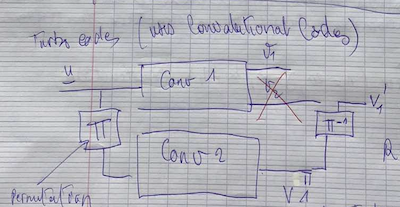
\includegraphics[keepaspectratio]{images/fig_turbo_codes.png}}
\caption{Figure (with permutations and Convolutions}
\end{figure}

    \begin{itemize}
\tightlist
\item
  Three Main powerful Codes

  \begin{itemize}
  \tightlist
  \item
    Turbo Codes \(\approx 1992\)
  \item
    LDPC Codes Gallager \(\approx 1960\)
  \item
    Polar Codes
  \end{itemize}
\item
  \textbf{All 3 codes achieve Capacity (\(\approx\)) with easier
  decoding}

  \begin{itemize}
  \tightlist
  \item
    LDPC easier to decode than Turbo
  \item
    Polar has smaller error decay (a little bit slower)
  \end{itemize}
\end{itemize}

\begin{center}\rule{0.5\linewidth}{0.5pt}\end{center}

    \section{\texorpdfstring{\textbf{Polar
Codes}}{Polar Codes}}\label{polar-codes}

\subsubsection{Notation:}\label{notation}

\begin{itemize}
\tightlist
\item
  \(X, Y \sim P_{X, Y}\): \[\begin{align}
      H(X) &= -\mathbb{E} \, \log P(X) \\
           &= -\sum_x P(x) \log P(x)
           \end{align}
  \]
\end{itemize}

Higher\(H\): More uncertainty

\begin{itemize}
\tightlist
\item
  \(H(X | Y)\): Joint Entropy
\item
  \(I(X; Y) = \underbrace{H(X)}_{10} - \underbrace{H(X | Y)}_{ - 7} \quad \underbrace{\textbf{= Mutual Information}}_\text{= 3 Bits of Information}\)
\end{itemize}

\subsection{\#\#\# Formulas:}\label{formulas}

\(\begin{align} H(X | Y) &\overset{\Delta}{=} -\mathbb{E}_{x,y} \, \log P(X | Y) \\ &= \sum_{x, y} P(x, y) \log \frac{1}{P(x | y)} \end{align}\)

\begin{itemize}
\item
  \(I(X; Y) = \sum\limits_{x, y} P(x, y) \log \frac{P(x, y)}{P(x) P(y)}\)
\item
  \(X^n = (X_1, \dots, X_n)\)
\item
  \(Y^n = (Y_1, \dots, Y_n)\)\(\qquad (X^n,Y^n) \sim P_{x^n,Y^n}\)
\end{itemize}

\subsubsection{Chain Rule:}\label{chain-rule}

\(\boxed{ H(X^n | Y^n) = \sum\limits_{i=1}^n H(X_i | Y^n, X^{i-1}) \; \textbf{ Where } \; X^{i-1} = (X_1, \dots, X_{i-1})}\)

    \(H(X_1 | Y^n) + H(X_2 | X_1, Y^n) + H(X_3 | \underbrace{X_1, X_2}_{(\because)}, Y^n) + \dots\)

\begin{quote}
\((\because)\) know the 2 previous days, (this is the chain rule).
\end{quote}

\(\begin{align} I(X^n; Y^n) &= \sum\limits_{i=1}^n I(X_i; Y^n | X^{i-1}) \\ &= I(X_1; Y_n) + I(X_2, Y_n| X_1) + \cdots \end{align}\)

    \textbf{Result (math)}

\subsubsection{Principle of
Polarization}\label{principle-of-polarization}

\begin{itemize}
\item
  Let \(X \sim P_X\), \(\mathcal{X} = \{0, 1\}\)
\item
  Let \(X_1, X_2, \dots\) i.i.d. \(\sim X\)
\item
  Let \(N = 2^n\), \(n > 1\)
\item
  Let \(X^n = \{X_1, X_2, \dots, X_n\}\)
\item
  Let: \(F = \begin{bmatrix} 1 & 0 \\ 1 & 1 \end{bmatrix}\),
  \(F^{\otimes n}\)= \(n\)-power Kronecker product of \(F\)
\end{itemize}

\(F^{\otimes 2} = \begin{bmatrix} 1 & 0 & 0 & 0 \\ 1 & 1 & 0 & 0 \\ 0 & 0 & 1 & 0 \\ 0 & 0 & 1 & 1 \end{bmatrix}\)

\(F^{\otimes 3} = \begin{bmatrix} 1 & 0 & 0 & 0 & 0 & 0 & 0 & 0 \\ 1 & 1 & 0 & 0 & 0 & 0 & 0 & 0 \\ 0 & 0 & 1 & 0 & 0 & 0 & 0 & 0 \\ 0 & 0 & 1 & 1 & 0 & 0 & 0 & 0 \\ 0 & 0 & 0 & 0 & 1 & 0 & 0 & 0 \\ 0 & 0 & 0 & 0 & 1 & 1 & 0 & 0 \\ 0 & 0 & 0 & 0 & 0 & 0 & 1 & 0 \\ 0 & 0 & 0 & 0 & 0 & 0 & 1 & 1 \end{bmatrix}\)

\begin{itemize}
\tightlist
\item
  Let \(u^N = x^N \cdot F^{\otimes n}\)
\end{itemize}

\subsubsection{Theorem:}\label{theorem}

\begin{itemize}
\item
  For any fixed \(\delta > 0\):
\item
  \(\boxed{\lim_{N \to \infty} \frac{1}{N} \left| \{ i \in \{1, 2, \dots, N\} \mid H(u_i | u^{i-1}) \in [\delta, 1-\delta] \} \right| = 0}\)
\item
  It says that:
  \(H(u_i | u^{i-1}) \to \begin{cases} 0       & \boxed{\text{ nothing in between them}} \\ 1 \end{cases}\)
\end{itemize}

    \pandocbounded{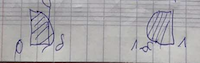
\includegraphics[keepaspectratio]{images/fig_no_uncertainty.png}}
\textbf{no uncertainty}

    \subsubsection{Polarization Kernel and Kronecker
Power}\label{polarization-kernel-and-kronecker-power}

\begin{enumerate}
\def\labelenumi{\arabic{enumi}.}
\item
  \textbf{Base Matrix \(F\):}
  \(F = \begin{bmatrix} 1 & 0 \\ 1 & 1 \end{bmatrix}\)
\item
  \textbf{Kronecker Power \(F^{\otimes n}\):}

  \begin{itemize}
  \tightlist
  \item
    Recursive definition:
    \(F^{\otimes n} = F^{\otimes (n-1)} \otimes F\)
  \item
    \(\otimes\): Kronecker product.
  \end{itemize}
\item
  \textbf{Examples:}

  \begin{itemize}
  \tightlist
  \item
    \(F^{\otimes 1} = F\)
  \item
    \(F^{\otimes 2}\):
    \(\begin{bmatrix} 1 & 1 & 0 & 0 \\ 1 & 0 & 0 & 0 \\ 1 & 1 & 1 & 1 \\ 1 & 0 & 1 & 0 \end{bmatrix}\)
  \item
    \(F^{\otimes 3}\):
    \(\begin{bmatrix} 1 & 0 & 0 & 0 & 0 & 0 & 0 & 0 \\ 1 & 1 & 0 & 0 & 0 & 0 & 0 & 0 \\ 0 & 0 & 1 & 0 & 0 & 0 & 0 & 0 \\ 0 & 0 & 1 & 1 & 0 & 0 & 0 & 0 \\ 0 & 0 & 0 & 0 & 1 & 0 & 0 & 0 \\ 0 & 0 & 0 & 0 & 1 & 1 & 0 & 0 \\ 0 & 0 & 0 & 0 & 0 & 0 & 1 & 0 \\ 0 & 0 & 0 & 0 & 0 & 0 & 1 & 1 \end{bmatrix}\)
  \end{itemize}
\item
  \textbf{Purpose:}

  \begin{itemize}
  \tightlist
  \item
    \(F^{\otimes n}\) transforms
    \(X^N \to U^N = X^N \cdot F^{\otimes n}\).
  \item
    Enables \textbf{channel polarization}, splitting channels into
    highly reliable and unreliable sets for polar codes.
  \end{itemize}
\end{enumerate}

    For any \(\delta > 0\), in fact \(\delta \approx 2^{-\sqrt{n}}\)\\
(i.e.~\(\delta\) can be as low as?)

\begin{center}\rule{0.5\linewidth}{0.5pt}\end{center}

\subsubsection{Example:}\label{example}

\begin{itemize}
\tightlist
\item
  \(n= 2, \; F = \begin{bmatrix} 1 & 0 \\ 1 & 1 \end{bmatrix}\)
\end{itemize}

\((u_1, u_2) = (x_1, x_2) \cdot  \begin{bmatrix} 1 & 0 \\ 1 & 1 \end{bmatrix} = \begin{bmatrix} x_1 \oplus x_2, x_2 \end{bmatrix}\)

\begin{itemize}
\tightlist
\item
  \(n = 4, \; F^{\otimes 2} = \begin{bmatrix} 10 & 00 \\ 11 & 00 \\ 10 & 10 \\ 11 & 11 \end{bmatrix}\)
\end{itemize}

\((u_1, u_2, u_3, u_4) = (x_1, x_2, x_3, x_4) \cdot F^{\otimes 2} = [ \underbrace{x_1 \oplus x_2 \oplus x_3 \oplus x_4}_{u_1} , \underbrace{x_2 \oplus x_4}_{u_2}  , \underbrace{x_3 \oplus x_4}_{u_3}  , \underbrace{x_4}_{u_4}  ]\)

\subsubsection{Kronecker Product:}\label{kronecker-product}

\(A = \begin{bmatrix} a_{11} & a_{12}  & \cdots \\ a_{21} & a_{22}s \\ \vdots \end{bmatrix}, B \qquad\)
\(A \otimes B = \begin{bmatrix} a_{11}B & a_{12}B \\ a_{21}B & \cdots \end{bmatrix}\)

\begin{center}\rule{0.5\linewidth}{0.5pt}\end{center}

    \subsubsection{\texorpdfstring{key result in \textbf{polar codes} and
\textbf{channel
polarization}}{key result in polar codes and channel polarization}}\label{key-result-in-polar-codes-and-channel-polarization}

\(x_1, x_2, \dots, x_n \qquad X \sim  \text{i.i.d.}\)

\(u^n = x^n \cdot F^n\)

\paragraph{Corollary:}\label{corollary}

\(\frac{\left[ \{ i : H(u_i | u^{i-1}) > 1 - \delta \} \right]}{N} = H(X)\)

\subsubsection{Proof:}\label{proof}

\(H(u^n) = H(x^n) = n \, H(x) (i.i.d)\)

This describes a key result in \textbf{polar codes} and \textbf{channel
polarization}, where the \textbf{entropy} and structure of the polar
transformation are analyzed mathematically.

\paragraph{Explanation:}\label{explanation}

\begin{enumerate}
\def\labelenumi{\arabic{enumi}.}
\tightlist
\item
  \textbf{Setup:}

  \begin{itemize}
  \tightlist
  \item
    \(x_1, x_2, \dots, x_n\): A sequence of independent and identically
    distributed (\textbf{i.i.d.}) random variables from the source
    \(X\).
  \item
    \(u^n = x^n \cdot F^n\): The transformation of \(x^n\) using the
    \textbf{Kronecker power} of \(F\) (polarization matrix) to produce
    the vector \(u^n\).

    \begin{itemize}
    \tightlist
    \item
      This defines the encoding operation in polar codes.
    \end{itemize}
  \end{itemize}
\item
  \textbf{Corollary:}

  \begin{itemize}
  \tightlist
  \item
    The fraction of indices \(i\) for which the \textbf{conditional
    entropy} \(H(u_i | u^{i-1}) > 1 - \delta\) (i.e., where uncertainty
    is high) is proportional to the \textbf{source entropy} \(H(X)\):
    \(\frac{\left| \{ i : H(u_i | u^{i-1}) > 1 - \delta \} \right|}{N} = H(X).\)
  \item
    This result demonstrates how the \textbf{polarization process}
    concentrates certain indices with high entropy (bad channels) and
    others with low entropy (good channels).
  \end{itemize}
\item
  \textbf{Proof Outline:}

  \begin{itemize}
  \tightlist
  \item
    Since \(x_1, x_2, \dots, x_n\) are i.i.d., the total entropy of the
    source sequence \(x^n\) is: \(H(x^n) = n \cdot H(X).\)
  \item
    The polar transformation preserves entropy (it's a linear
    transformation), so: \(H(u^n) = H(x^n) = n \cdot H(X).\)
  \item
    This shows that the entropy is distributed across the components of
    \(u^n\), leading to the polarization effect.
  \end{itemize}
\end{enumerate}

\paragraph{Key Idea:}\label{key-idea}

\begin{itemize}
\tightlist
\item
  \textbf{Channel Polarization}:

  \begin{itemize}
  \tightlist
  \item
    The transformation \(F^n\) polarizes the ``channels'' (indices
    \(i\)) into two categories:

    \begin{enumerate}
    \def\labelenumi{\arabic{enumi}.}
    \tightlist
    \item
      Channels with \textbf{high reliability}
      (\(H(u_i | u^{i-1}) \approx 0\)): These are the ``good'' channels
      used to carry information.
    \item
      Channels with \textbf{low reliability}
      (\(H(u_i | u^{i-1}) \approx 1\)): These are the ``bad'' channels,
      which are ``frozen'' (fixed to known values).
    \end{enumerate}
  \end{itemize}
\item
  The corollary quantifies this polarization, stating that the fraction
  of good channels corresponds to the source entropy \(H(X)\).
\end{itemize}

\paragraph{Summary:}\label{summary}

\begin{itemize}
\tightlist
\item
  \textbf{Transformation}: \(u^n = x^n \cdot F^n\) is the polar
  transformation.
\item
  \textbf{Result}: The fraction of ``good'' channels (low-entropy)
  matches the source entropy \(H(X)\).
\item
  \textbf{Proof}: Entropy is conserved, and the polarization process
  redistributes it across the indices of \(u^n\).
\end{itemize}

This result is central to the design and analysis of \textbf{polar
codes}, enabling efficient encoding and decoding.

    \begin{center}\rule{0.5\linewidth}{0.5pt}\end{center}

\(H(u^N) = \sum\limits_{i=1}^N \underbrace{H(u_i | u^{i-1})}_\text{(chain rule)} \quad  = N \cdot H(X)\)\((\because)\)

But recall (from theorem) that the \# of terms where:
\(H(u_i | u^{i-1}) \in (\delta, 1-\delta) \quad \text{is near zero.}\)

\(\approx 0 \cdot \Big| \overbrace{H(u_i | u^{i-1})}^{\# \text{of times }} \approx 0 \Big| + 1 \cdot \Big| \overbrace{H(u_i | u^{i-1})}^{\# \text{of times }} \approx 1 \Big|\)

All the entropy accumulated in summation is due to \(K\) terms where:
\(H(u_i | u^{i-1}) \in (1 - \delta, 1).\)

\subsubsection{Accumulated Entropy:}\label{accumulated-entropy}

\(K \cdot 1 = N \cdot H(X) \quad (\text{from }\because) \implies \frac{K}{N} = H(X).\)

\(H(X) \approx 0.3 \qquad \text{30\% of } H(u_i | u^{i-1}) \approx 1's, \quad 70\% \approx 0.\)

\begin{figure}
\centering
\pandocbounded{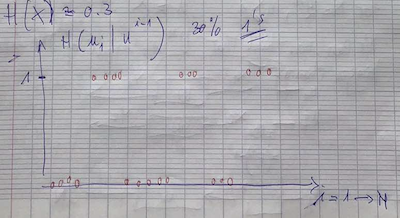
\includegraphics[keepaspectratio]{images/fig_accumulated_entropy.png}}
\caption{accumulated entropy}
\end{figure}

\begin{figure}
\centering
\pandocbounded{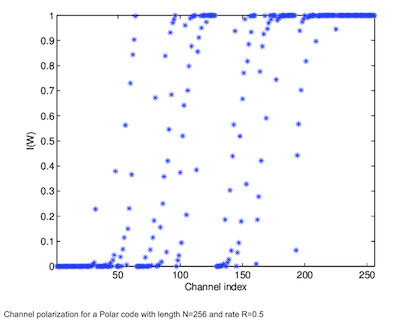
\includegraphics[keepaspectratio]{images/fig_channel_polarization.png}}
\caption{channel polarization}
\end{figure}

\paragraph{\texorpdfstring{Explanation of
\(K \cdot 1 = N \cdot H(X) \implies \frac{K}{N} = H(X)\)}{Explanation of K \textbackslash cdot 1 = N \textbackslash cdot H(X) \textbackslash implies \textbackslash frac\{K\}\{N\} = H(X)}}\label{explanation-of-k-cdot-1-n-cdot-hx-implies-frackn-hx}

This equation arises in the context of \textbf{polar codes} and
\textbf{channel polarization}, describing how the total entropy is
distributed among the indices of the polar transformation.

\begin{center}\rule{0.5\linewidth}{0.5pt}\end{center}

\paragraph{Definitions and Context:}\label{definitions-and-context}

\begin{enumerate}
\def\labelenumi{\arabic{enumi}.}
\tightlist
\item
  \textbf{Terms}:

  \begin{itemize}
  \tightlist
  \item
    \(K\): The number of indices \(i\) where the \textbf{conditional
    entropy} \(H(u_i | u^{i-1})\) contributes meaningfully to the total
    entropy (i.e., \(H(u_i | u^{i-1}) \approx 1\)).
  \item
    \(N\): The total block length (number of indices in \(u^N\)).
  \item
    \(H(X)\): The entropy of the source variable \(X\), which determines
    the overall proportion of good (reliable) channels in the
    polarization process.
  \end{itemize}
\item
  \textbf{Accumulated Entropy}:

  \begin{itemize}
  \tightlist
  \item
    The total entropy of the transformed vector \(u^N\) is:
    \(H(u^N) = N \cdot H(X),\) since entropy is preserved during the
    linear transformation \(u^N = x^N \cdot F^N\).
  \end{itemize}
\end{enumerate}

\paragraph{Key Idea:}\label{key-idea}

\begin{itemize}
\tightlist
\item
  \textbf{Entropy Contribution}:

  \begin{itemize}
  \tightlist
  \item
    The entropy \(H(u^N)\) is primarily accumulated in the \(K\) terms
    where \(H(u_i | u^{i-1}) \approx 1\) (good channels).
  \item
    For other indices, \(H(u_i | u^{i-1}) \approx 0\), meaning they
    contribute negligible entropy.
  \end{itemize}
\item
  \textbf{Total Accumulated Entropy}:

  \begin{itemize}
  \tightlist
  \item
    If \(K\) terms contribute nearly \(1\) unit of entropy each, the
    total entropy contributed by these terms is:
    \(K \cdot 1 = N \cdot H(X).\)
  \end{itemize}
\item
  \textbf{Proportion of Good Channels}:

  \begin{itemize}
  \tightlist
  \item
    Dividing through by \(N\), we find that the proportion of indices
    \(i\) where \(H(u_i | u^{i-1}) \approx 1\) is:
    \(\frac{K}{N} = H(X).\)
  \end{itemize}
\end{itemize}

\paragraph{Meaning:}\label{meaning}

\begin{itemize}
\tightlist
\item
  \(\frac{K}{N} = H(X)\) indicates that the fraction of ``good
  channels'' (indices \(i\) where \(H(u_i | u^{i-1})\) is significant)
  corresponds to the source entropy \(H(X)\).
\item
  For example:

  \begin{itemize}
  \tightlist
  \item
    If \(H(X) = 0.3\), then 30\% of the channels are reliable, while
    70\% are unreliable (contributing \(H(u_i | u^{i-1}) \approx 0\)).
  \end{itemize}
\end{itemize}

\paragraph{Importance in Polar Codes:}\label{importance-in-polar-codes}

This relationship quantifies \textbf{channel polarization}, where: - A
fraction \(H(X)\) of the channels becomes highly reliable (used for
transmitting information). - The remaining fraction \(1 - H(X)\) becomes
unreliable (frozen).

This ensures that polar codes can efficiently encode and decode data
based on the structure of \(F^N\).

    \begin{center}\rule{0.5\linewidth}{0.5pt}\end{center}

\subsubsection{Channel Polarization}\label{channel-polarization}

\(X \to \boxed{ W } \to Y\)\(\qquad X\)is Input to the memoryless
channel\(W\).

\textbf{Recall}: \((x, y) \sim P_{X,Y}(x, y)\)

\[
\begin{align}
P(X, Y) &= P_X(x) \cdot P_{Y|X}(y|x) \\
        &= P_X(x) \cdot W_{Y|X}(y|x)
\end{align}
\]

Using Bayes' Rule:
\(P_{X|Y}(x|y) = \frac{P_{Y|X}(y|x) \cdot P_X(x)}{P_Y(y)} \quad \text{(Channel Fixed)}.\)

\begin{center}\rule{0.5\linewidth}{0.5pt}\end{center}

\textbf{Assume}: - \(X \sim X_1, X_2, \dots, X_n\),\\
- \(X\) is discrete, \(X \in \{0, 1\}\),\\
- Assume Binary Symmetric Channel (BSC).

For \(N = 2^n\): \(U^N = X^N \cdot F^n\) \(U^N\): Input of the following
\textbf{bigger channel}:

\begin{center}\rule{0.5\linewidth}{0.5pt}\end{center}

\subsubsection{Diagram:}\label{diagram}

\begin{itemize}
\tightlist
\item
  \(W\): Memoryless channel,
\item
  \(U_1, U_2, \dots, U_N\): Input,
\item
  \(Y_1, Y_2, \dots, Y_N\): Output.
\end{itemize}

This process \textbf{creates bad and good channels}, enabling
\textbf{channel polarization}.

    \paragraph{\texorpdfstring{\textbf{1. Singleton
Bound:}}{1. Singleton Bound:}}\label{singleton-bound}

The \textbf{Singleton bound} is a theoretical limit in coding theory
that relates the code length, code rate, and minimum distance of a block
code. It sets a limit on the trade-off between error correction and code
efficiency.

\subparagraph{\texorpdfstring{\textbf{Definition:}}{Definition:}}\label{definition}

For a block code with parameters \([n, k, d]\): - \(n\): Codeword
length. - \(k\): Number of information symbols. - \(d\): Minimum Hamming
distance between any two distinct codewords.

The \textbf{Singleton bound} states: \(d \leq n - k + 1\)

This means that for a code of length \(n\) and \(k\) information
symbols, the minimum distance \(d\) cannot exceed \(n - k + 1\).

\paragraph{\texorpdfstring{\textbf{2. MDS Codes (Maximum Distance
Separable
Codes):}}{2. MDS Codes (Maximum Distance Separable Codes):}}\label{mds-codes-maximum-distance-separable-codes}

A code that achieves the Singleton bound with equality is called an
\textbf{MDS (Maximum Distance Separable) code}.

\subparagraph{\texorpdfstring{\textbf{Definition:}}{Definition:}}\label{definition-1}

A block code is called an MDS code if: \(d = n - k + 1\)

MDS codes have the \textbf{maximum possible minimum distance} for their
given length \(n\) and dimension \(k\).

\paragraph{\texorpdfstring{\textbf{Properties of MDS
Codes:}}{Properties of MDS Codes:}}\label{properties-of-mds-codes}

\begin{enumerate}
\def\labelenumi{\arabic{enumi}.}
\item
  \textbf{Error correction and detection:}

  \begin{itemize}
  \tightlist
  \item
    An MDS code can correct up to \(\lfloor \frac{d - 1}{2} \rfloor\)
    errors.
  \item
    It can detect up to \(d - 1\) errors.
  \end{itemize}
\item
  \textbf{Examples of MDS Codes:}

  \begin{itemize}
  \tightlist
  \item
    \textbf{Reed-Solomon codes}: Widely used in communication systems
    (e.g., CDs, DVDs, and QR codes).
  \item
    \textbf{Simple parity check codes}: (e.g., \([n, n-1, 2]\)), which
    can detect a single error.
  \item
    \textbf{Repetition codes}: (e.g., \([n, 1, n]\)), which repeat the
    same symbol multiple times.
  \end{itemize}
\item
  \textbf{Generator Matrix Properties:} For an MDS code, any
  \(k \times k\) submatrix of the generator matrix is invertible.
\item
  \textbf{Dual Codes}: The dual of an MDS code is also MDS, with
  parameters \([n, n-k, k+1]\).
\end{enumerate}

\paragraph{\texorpdfstring{\textbf{Example: Reed-Solomon
Code}}{Example: Reed-Solomon Code}}\label{example-reed-solomon-code}

For a \textbf{Reed-Solomon} code with parameters \([n, k, d]\): -
\(n = q - 1\) (over a finite field of size \(q\)), - \(d = n - k + 1\),
which achieves the Singleton bound.

This is why Reed-Solomon codes are essential in applications where
robust error correction is needed.

\paragraph{\texorpdfstring{\textbf{Summary:}}{Summary:}}\label{summary}

\begin{itemize}
\tightlist
\item
  The \textbf{Singleton bound} defines an upper limit on the minimum
  distance of a block code.
\item
  \textbf{MDS codes} achieve this limit and have the highest error
  correction capabilities for a given code length and dimension.
\end{itemize}

    \paragraph{\texorpdfstring{\textbf{Numerical Problem: Singleton Bound
and MDS
Code}}{Numerical Problem: Singleton Bound and MDS Code}}\label{numerical-problem-singleton-bound-and-mds-code}

A communication system uses a block code with the following parameters:
- Code length \(n = 10\), - Number of information symbols \(k = 6\).

\begin{enumerate}
\def\labelenumi{\arabic{enumi}.}
\tightlist
\item
  \textbf{Calculate the Singleton bound} for this code.
\item
  If the code has a minimum distance \(d = 5\), is this code an MDS
  code?
\item
  Determine how many errors this code can \textbf{correct} and
  \textbf{detect}.
\end{enumerate}

\paragraph{\texorpdfstring{\textbf{Solution
Steps:}}{Solution Steps:}}\label{solution-steps}

\subparagraph{\texorpdfstring{\textbf{Step 1: Singleton Bound
Calculation}}{Step 1: Singleton Bound Calculation}}\label{step-1-singleton-bound-calculation}

The Singleton bound is given by: \(d \leq n - k + 1\)

Substitute \(n = 10\) and \(k = 6\) into the formula:
\(d \leq 10 - 6 + 1 = 5\)

Thus, the Singleton bound for this code is \textbf{5}.

\subparagraph{\texorpdfstring{\textbf{Step 2: Check if the code is
MDS}}{Step 2: Check if the code is MDS}}\label{step-2-check-if-the-code-is-mds}

The code has \(d = 5\), which equals the Singleton bound. Therefore, the
code \textbf{achieves the Singleton bound} and is an \textbf{MDS code}.

\subparagraph{\texorpdfstring{\textbf{Step 3: Error Correction and
Detection}}{Step 3: Error Correction and Detection}}\label{step-3-error-correction-and-detection}

For an MDS code with \(d = 5\):

\begin{enumerate}
\def\labelenumi{\arabic{enumi}.}
\item
  \textbf{Error correction capability:} The number of errors the code
  can correct is:
  \(t = \left\lfloor \frac{d - 1}{2} \right\rfloor = \left\lfloor \frac{5 - 1}{2} \right\rfloor = \left\lfloor 2 \right\rfloor = 2\)

  So, the code can correct \textbf{2 errors}.
\item
  \textbf{Error detection capability:} The code can detect up to
  \textbf{\(d - 1 = 4\)} errors.
\end{enumerate}

\paragraph{\texorpdfstring{\textbf{Final
Answers:}}{Final Answers:}}\label{final-answers}

\begin{enumerate}
\def\labelenumi{\arabic{enumi}.}
\tightlist
\item
  Singleton bound: \(d \leq 5\),
\item
  The code is an \textbf{MDS code} since \(d = 5\),
\item
  The code can correct \textbf{2 errors} and detect \textbf{4 errors}.
\end{enumerate}

    \paragraph{\texorpdfstring{\textbf{Sphere Packing Bound in Coding
Theory}}{Sphere Packing Bound in Coding Theory}}\label{sphere-packing-bound-in-coding-theory}

The \textbf{sphere packing bound} (also known as the \textbf{Hamming
bound}) gives a limit on how many codewords can fit in a Hamming space
without their \textbf{error correction spheres} overlapping. It connects
the \textbf{packing radius}, \textbf{covering radius}, and code
parameters like the minimum distance \(d\).

\subsubsection{\texorpdfstring{\textbf{Formal Statement of the
Bound:}}{Formal Statement of the Bound:}}\label{formal-statement-of-the-bound}

For a block code with parameters \([n, k, d]\), where: - \(n\): Codeword
length, - \(k\): Number of information symbols (dimension of the code),
- \(d\): Minimum distance between codewords, -
\(t = \lfloor (d-1)/2 \rfloor\): Error correction radius (packing
radius),

The sphere packing bound is: \(M \cdot V(t, n) \leq 2^n\)

Where: - \(M = 2^k\) is the number of codewords. - \(V(t, n)\) is the
volume of a Hamming ball of radius \(t\), given by:
\(V(t, n) = \sum_{i=0}^{t} \binom{n}{i}\)

\paragraph{\texorpdfstring{\textbf{Explanation:}}{Explanation:}}\label{explanation}

\begin{itemize}
\tightlist
\item
  The \textbf{packing radius} \(t\) defines the maximum number of errors
  a code can correct.
\item
  Each codeword has a Hamming sphere of radius \(t\).
\item
  The total volume occupied by these spheres must not exceed the size of
  the entire Hamming space, \(2^n\).
\item
  This constraint limits the maximum number of codewords \(M\), ensuring
  no overlapping.
\end{itemize}

\paragraph{\texorpdfstring{\textbf{Perfect Codes and the Sphere Packing
Bound:}}{Perfect Codes and the Sphere Packing Bound:}}\label{perfect-codes-and-the-sphere-packing-bound}

A \textbf{perfect code} achieves equality in the sphere packing bound:
\(M \cdot V(t, n) = 2^n\)

This means that: 1. The code's \textbf{error spheres} fill the Hamming
space exactly, without gaps or overlaps. 2. For perfect codes, the
\textbf{covering radius} \(R\) equals the \textbf{packing radius} \(t\).

\paragraph{\texorpdfstring{\textbf{Example: Hamming
Code}}{Example: Hamming Code}}\label{example-hamming-code}

Consider a Hamming code with parameters \([7, 4, 3]\): - \(n = 7\),
\(k = 4\), \(d = 3\), and \(t = 1\). - The volume of a Hamming sphere
with radius \(t = 1\) is:
\(V(1, 7) = \binom{7}{0} + \binom{7}{1} = 1 + 7 = 8\) - The number of
codewords is \(M = 2^k = 16\).

Check the sphere packing bound:
\(M \cdot V(1, 7) = 16 \cdot 8 = 128 = 2^7\)

Since equality holds, the Hamming code is a \textbf{perfect code}.

\paragraph{\texorpdfstring{\textbf{Relationship
Recap:}}{Relationship Recap:}}\label{relationship-recap}

\begin{longtable}[]{@{}
  >{\raggedright\arraybackslash}p{(\linewidth - 2\tabcolsep) * \real{0.2391}}
  >{\raggedright\arraybackslash}p{(\linewidth - 2\tabcolsep) * \real{0.7609}}@{}}
\toprule\noalign{}
\begin{minipage}[b]{\linewidth}\raggedright
\textbf{Concept}
\end{minipage} & \begin{minipage}[b]{\linewidth}\raggedright
\textbf{Definition}
\end{minipage} \\
\midrule\noalign{}
\endhead
\bottomrule\noalign{}
\endlastfoot
\textbf{Packing Radius} \(t\) & Radius where spheres around codewords do
not overlap (related to error correction). \\
\textbf{Covering Radius} \(R\) & Maximum radius needed to cover all
vectors in the Hamming space. \\
\textbf{Sphere Packing Bound} & \(M \cdot V(t, n) \leq 2^n\), limits
maximum codewords without sphere overlap. \\
\textbf{Perfect Code} & Achieves equality in the sphere packing bound,
with \(R = t\). \\
\end{longtable}

\paragraph{\texorpdfstring{\textbf{1. Covering Radius
\(R\)}}{1. Covering Radius R}}\label{covering-radius-r}

Let \(C\) be a code with codewords
\(\underline{c}_1, \underline{c}_2, \dots, \underline{c}_M\), where
\(M\) is the number of codewords, and let \(F_2^n\) be the
\textbf{Hamming space} of dimension \(n\). Define the Hamming ball
centered at a codeword \(\underline{c}\) with radius \(r\) as:
\(\text{Ball}(\underline{c}, r) = \{ v \in F_2^n \mid d_H(v, \underline{c}) \leq r \}\)

The \textbf{covering radius} \(R\) is the smallest radius such that the
union of all balls centered at codewords covers the entire space:
\(R = \min \{ r \mid \bigcup_{\underline{c} \in C} \text{Ball}(\underline{c}, r) = F_2^n \}\)

This means that every vector in \(F_2^n\) lies within radius \(R\) of
some codeword in \(C\).

\paragraph{\texorpdfstring{\textbf{2. Packing Radius \(S\) (Error
Correction
Radius)}}{2. Packing Radius S (Error Correction Radius)}}\label{packing-radius-s-error-correction-radius}

The \textbf{packing radius} \(t\) is the largest radius for which balls
centered at distinct codewords do not overlap. Formally:
\(t = \max \{ r \mid \text{Ball}(\underline{c}_i, r) \cap \text{Ball}(\underline{c}_j, r) = \emptyset, \, \forall \, \underline{c}_i \neq \underline{c}_j \in C \}\)

This ensures that no two balls of radius \(t\) around different
codewords intersect, allowing for error correction up to \(t\) errors.

In simpler terms, the packing radius is:
\(t = \left\lfloor \frac{d - 1}{2} \right\rfloor\) where \(d\) is the
minimum Hamming distance between any two codewords in \(C\).

\paragraph{\texorpdfstring{\textbf{Key Relationship (Perfect
Codes):}}{Key Relationship (Perfect Codes):}}\label{key-relationship-perfect-codes}

For \textbf{perfect codes}, the packing radius \(t\) and covering radius
\(R\) are equal: \(R = t\)

\paragraph{\texorpdfstring{\textbf{Summary:}}{Summary:}}\label{summary}

\begin{itemize}
\tightlist
\item
  The \textbf{covering radius} is the smallest radius where all vectors
  in the Hamming space are within some ball centered on a codeword.
\item
  The \textbf{packing radius} is the largest radius where no two balls
  around different codewords overlap.
\item
  Perfect codes achieve \(R = t\).
\end{itemize}

    \paragraph{In Phone}\label{in-phone}

outerspace: AWGN \(y = x + w\)

\begin{itemize}
\item
  ``closed library night'' (SIMO)
  \(\qquad y = \underline{h} \, \underline{x} + w\) but
  \(\underline{h}, \underline{x}, w\) \(\forall\) fixed (and generally
  known)
\item
  \(C_{\text{simo}} = \log(1 + \rho |h|^2)\) LTI
  \(\qquad \underline{y} = \underline{h} \, x + w\)

  \begin{itemize}
  \tightlist
  \item
    rx beamforming (CSIR)
  \end{itemize}
\item
  \(C_{\text{miso}} = \log(1 + \rho |\underline{h}|^2)\) CSITR
  \(\qquad y_i = H \cdot \underline{x} + \underline{w}\)
\item
  ``outside''
\end{itemize}

CSIT is hard to get \(y = h + w\) but \(h_i \sim\) randomly chosen

\begin{itemize}
\tightlist
\item
  Quasi Static Fading (≠ diversity Techniques ST code)
\item
  Fast fading \(\qquad C_{\text{FF}} = C_{\text{AWGN}}\)
\end{itemize}

\(\boxed{\text{channel is chosen (drawn) randomly but here to stay}}\)

    \begin{tcolorbox}[breakable, size=fbox, boxrule=1pt, pad at break*=1mm,colback=cellbackground, colframe=cellborder]
\prompt{In}{incolor}{ }{\boxspacing}
\begin{Verbatim}[commandchars=\\\{\}]

\end{Verbatim}
\end{tcolorbox}


    % Add a bibliography block to the postdoc
    
    
    
\end{document}
